\documentclass[a4paper,12pt]{article}

\usepackage[utf8]{inputenc}
\usepackage[english,russian]{babel}
\usepackage{longtable}
\usepackage{amsmath}
\usepackage{amsfonts}
\usepackage{amssymb}
\usepackage{cite}
\usepackage{graphicx}
\usepackage{epstopdf}
\usepackage{datetime}
\usepackage{indentfirst}
\usepackage{subfigure}
\usepackage[section]{placeins}
\usepackage{afterpage}
\usepackage{url}
\usepackage[unicode]{hyperref}
\usepackage{ucs}
\usepackage{listings}
\usepackage{microtype}
\usepackage{paralist}
\usepackage{multirow}
\usepackage{color}
\usepackage{xcolor}
\usepackage{float}
\usepackage{graphicx}
\usepackage{sectsty}
\usepackage{fancyhdr}
\usepackage{longtable}
\usepackage{appendix}
\usepackage{enumerate}
\usepackage{totcount}
\usepackage{verbments}
\usepackage{perpage}
\usepackage{caption}
\usepackage{varwidth}
\usepackage{listings}
\usepackage{listingsutf8}

\newfloat{floatquote}{tbp}{loq}
\floatname{floatquote}{Цитата}
%\captionsetup{font =small, format = hang}
\usepackage{cleveref}
\crefname{floatquote}{quote}{quotes}
\Crefname{floatquote}{Quote}{Quotes}
\DeclareFontShape{OT1}{cmtt}{bx}{n}{<5><6><7><8><9><10><10.95><12><14.4><17.28><20.74><24.88>cmttb10}{}

\makeatletter
\renewcommand{\@biblabel}[1]{#1.}
\makeatother

\usepackage{geometry}
\geometry{left=2cm}
\geometry{right=2cm}
\geometry{top=2cm}
\geometry{bottom=2cm}

%% from bachelor-paper begin 
\fancyhf{}
\fancyfoot[C]{\normalsize \thepage}
\renewcommand{\headrulewidth}{0pt}
\renewcommand{\footrulewidth}{0pt}

%%Modifying captions for figures and tables:
%\makeatletter
%\long\def\@makecaption#1#2{%
%\vspace{\abovecaptionskip}%
%\sbox{\@tempboxa}{\large #1.~#2}
%\ifdim \wd\@tempboxa >\hsize
%% {\normalsize #1 --- #2}\par
%\global\@minipagefalse
%\hbox to \hsize {\hfill {\normalsize #1 --- #2}\hfill}%
%\else
%% {\normalsize #1 --- #2}\par
%\global\@minipagefalse
%\hbox to \hsize {\hfill {\normalsize #1 --- #2}\hfill}%
%\fi
%\vspace{\belowcaptionskip}}

\DeclareCaptionFormat{myformat}{%
    % #1: label (e.g. "Table 1")
    % #2: separator (e.g. ": ")
    % #3: caption text
    \begin{varwidth}{\linewidth}%
        \centering
        #1 --- #3%
    \end{varwidth}%
}
\captionsetup{format=myformat}% global activation

\makeatletter
\providecommand{\bigsqcap}{%
\mathop{%
\mathpalette\@updown\bigsqcup
}%
}
\newcommand*{\@updown}[2]{%
\rotatebox[origin=c]{180}{$\m@th#1#2$}%
}
\makeatother

%% replaced with linespread? \renewcommand{\baselinestretch}{1.2}
\sectionfont{\Large}
\subsectionfont{\Large}
\subsubsectionfont{\Large}
\setlength{\belowcaptionskip}{6pt}
%% \makeatletter \renewcommand{\@biblabel}[1]{#1.\hfill}

\makeatletter 
\def\redeflsection{\def\l@section{\@dottedtocline{1}{1.5em}{7.8em}}} 
\renewcommand\appendix{\par 
\setcounter{section}{0}% 
\setcounter{subsection}{0}% 
\def\@chapapp{\appendixname}% 
\addtocontents{toc}{\protect\redeflsection} 
\def\thesection{\appendixname\hspace{0.2cm}\@Asbuk\c@section}} 
\makeatother 

\textwidth = 17cm
\oddsidemargin= 0 pt
\topmargin = -1cm
\headheight = 0cm
\headsep = 0cm
\textheight = 26.5cm

\newtotcounter[auxfile=totals.aux]{figurecnt}
\def\oldfigure{} \let\oldfigure=\figure
\def\figure{\stepcounter{figurecnt}\oldfigure}
\newtotcounter[auxfile=totals.aux]{bibcnt}
\def\oldbibitem{} \let\oldbibitem=\bibitem
\def\bibitem{\stepcounter{bibcnt}\oldbibitem}
\regtotcounter[auxfile=totals.aux]{page}

\linespread{1.3}

\newcommand{\td}{ (\#TODO) }
\newcommand{\todo}[1]{(\#TODO: #1)}
\newcommand{\doubletext}[2]{
	\noindent\begin{minipage}[b]{0.5\linewidth}
        #1
	\end{minipage}
	\noindent\begin{minipage}[b]{0.45\linewidth}
        \begin{flushright}
            #2
        \end{flushright}
    \end{minipage}
}

%\renewcommand{\theenumi}{\arabic{enumi}}
%\renewcommand{\labelenumi}{\arabic{enumi}}
%\renewcommand{\theenumii}{.\arabic{enumii}}
%\renewcommand{\labelenumii}{\arabic{enumi}.\arabic{enumii}.}
%\renewcommand{\theenumiii}{.\arabic{enumiii}}
%\renewcommand{\labelenumiii}{\arabic{enumi}.\arabic{enumii}.\arabic{enumiii}.}

\floatstyle{plain} % optionally change the style of the new float
\newfloat{code}{H}{myc}

\newcommand{\fu}[1]{\footnote{\url{#1}}}

%\definecolor{javapurple}{rgb}{0.25,0.35,0.9} % keywords
%% \definecolor{javapurple}{rgb}{0.1,0.1,0.1}


%\lstset{
%captionpos=b,
%breaklines=true,
%% basicstyle=\ttfamily,
%keywordstyle=\bfseries,
%% keywordstyle=\color{javapurple}\bfseries,
%% basicstyle=\ttfamily\color{black},
%% keywordstyle=\bfseries\color{keyword},
%showstringspaces=false,
%morekeywords={fun, val, var, import, object, uses, classpath, let, for, do, select, in, return, new, null, class}
%}

\MakePerPage{footnote}

\begin{document}
\lstset{
    inputencoding=utf8,
    language=Pascal
}
\def\figurename{Рисунок}

\begin{titlepage}
\large
\newpage

\begin{center}
Федеральное государственное бюджетное \\
образовательное учреждение высшего образования \\
Санкт-Петербургский национальный \\
исследовательский академический университет \\
российской академии наук
\end{center}

\begin{flushright}
\begin{minipage}[t][12em][c]{30ex}
\begin{center}
На правах рукописи \\
\medskip
Диссертация допущена к защите \\
Зав. кафедрой \\
\hrulefill \\
<<\hspace{2em}>> \hspace{1ex} \hrulefill \hspace{1ex} 2015 г.\\
\end{center}
\end{minipage}
\end{flushright}

\begin{center}
Диссертация \\
на соискание ученой степени \\
магистра \\
\end{center}

\noindent{Тема: Оптимизация байт-кода, генерируемого компилятором Kotlin}

\vspace{0.5cm}

\noindent{Направление: 03.04.01    –  Прикладные математика и физика}

\vspace{1.5cm}

\doubletext{Выполнил студент}{Д.С. Жарков}
\begin{center}
    \small (подпись)
\end{center}

\vspace{0.2cm}

\doubletext{Руководитель:}{А.А. Бреслав}
\begin{center}
    \small (подпись)
\end{center}

\vspace{0.2cm}

\doubletext{Рецензент: \\ к.ф.-м.н., доцент}{}
\begin{center}
    \small (подпись)
\end{center}

\vspace{1cm}

\begin{center}
    Санкт-Петербург

    2015 г.
\end{center}

\normalsize
\end{titlepage}


\addcontentsline{toc}{section}{Содержание}
\tableofcontents

\clearpage
\section*{Введение}
\addcontentsline{toc}{section}{\hspace{7mm}Введение}

Язык программирования Java на сегодняшний день является одним из самых популярных инструментов
разработки программного обеспечения. \footnote{\url{http://langpop.com/}}

Во многом своей популярности он обязан платформе JRE (Java Runtime Environment), включающей в себя
стандартную библиотеку языка и виртуальную машину Java (JVM), на которой исполняется скомпилированный код.
Именно наличие последнего пункта значительно облегчает задачу разработчика, решая такие непростые
проблемы,  как кросплатформенность, безопасность, управление памятью и отчасти производительность ПО.

Однако сам язык Java обладает рядом существенных недостатков: многословный и ``бедный'' синтаксис,
слабый вывод типов, развитие языка заторможено необходимостью сохранять обратную совместимость.

В связи с этим на рынке появляются новые языки, преодолевающие эти недостатки, но также
компилирующие исходный код программ в байткод для JVM и сохраняющие таким образом преимущества платформы.
Примером таких языков могут послужить Groovy, Scala, Kotlin, Clojure, Ceylon.

Поскольку для решений, базирующихся на платформе Java, нередко критичным фактором является
производительность и размер байткода приложения, то при сравнении этих языков в том числе следует
учитывать эти параметры кода, генерируемого их компиляторами.

Kotlin разрабатывается в компании JetBrains с 2010 года, а выпуск первой версии запланирован на середину 2015 года.

В рамках данной работы будет произведен анализ производительности байткода генерируемого его транслятором,
а также описаны решения, принятые для устранения найденных недочетов, такие как:
\begin{itemize}
    \item Устранение избыточного боксинга.
    \item Оптимизация генерации кода для сочетания операторов безопасного вызова и ``Elvis''.
    \item Оптимизация генерации оператора ``when'' для целочисленных констант, строк и классов-перечислений.
    \item Удаление мертвого кода.
    \item Решение проблемы с нарушением условий для <<On-stack-replacement>>.
\end{itemize}

%Квалификационная работа состоит из двух глав.

%В первой главе рассмотрены основные понятия предметной области, а также детализированы цели и задачи данной работы.

%Во второй рассмотрены уже существующие решения и приведены детали реализации полученной в рамках данной работы системы.

%В заключении описаны результаты работы и сформулированы перспективы дальнейшего развития системы.

\clearpage

\section*{Постановка задачи}

Главной целью данной работы --- улучшение производительности байт-кода, генерируемого компилятором
Kotlin.

Для ее достижения необходимо было решить следующие задачи:
\begin{itemize}
    \item Изучение подходов к производительности кода, реализованных в компиляторах других
    языков программирования для платформы Java.

    \item Измерение производительности байт-кода, генерируемого компилятором для различных
    синтаксических конструкций.

    \item Анализ, трактовка и классификация найденных в рамках стадии измерения проблем.

    \item Исследование оптимизаций, проводимых современными реализациями виртуальной машины
    Java, необходимое для определения критичности найденных проблем в генерируемом коде.

    \item Внедрение в компилятор изменений, способствующих решению найденных недостатков в коде
    и измерение производительности после этих изменений.
\end{itemize}

\clearpage

\section{Обзор предметной области}

\subsection{Виртуальная машина Java}

В этом разделе будет описан ряд особенностей, с которыми сталкиваются разработчики языков
программирования,компилирующихся в байткод виртуальной машины Java, далее именуемой \textit{JVM}.

В первую очередь следует подчеркнуть, что JVM --- абстрактная виртуальная машина, работающая
в соответствии со официальной спецификацией, выпущенной компанией Sun Microsystems и ныне
принадлежащей компании Oracle. %% spec link in biblio

У нее существует множество реализаций, в разной степени удовлетворяющих требованиям спецификации.
Известными примерами могут послужить: \textit{Hotspot} и \textit{JRockit} от Oracle, \textit{Azul Zing}
и \textit{Azul Zulu} --- относительно новые реализации от компании Azul Systems, \textit{Apache Harmony},
и многие другие.

\paragraph{Байт-код}

Основной сущностью, с которой работает JVM, является так называемый <<class-файл>>, как правило являющийся
бинарным отражением отдельного класса из исходного кода на языке Java. В нем закодированы основные
характеристики класса, такие как набор полей и методов, информация о его происхождении --- имя
скомпилированного файла, набор используемых строковых констант, и многое другое.

В рамках описания отдельного метода наиболее важной его частью является непосредственно код --- список
инструкций, которые должны быть исполнены виртуальной машиной при вызове этого метода.

Стоит отдельно упомянуть об особенностях набора инструкций JVM, существенно отличающих его
от низкоуровневых наборов, таких как x86 или ARM, которые реализованы для большинства современных
процессоров:
\begin{enumerate}
    \item Интерпретатор JVM представляет собой стековую машину, то есть операнды инструкций, как и
    их результаты, располагаются на стеке, причем в рамках работы одного вызова метода
    нельзя получить доступ к стеку родительского вызова.
    \item В наборе инструкций отсутствуют механизмы для ``прямого'' доступа к памяти процесса, по
    спецификации JVM состояние программы исчерпывается содержимым локальных переменных вызовов,
    полей объектов и статических полей классов.
    \item Единственным способом интерпроцедурного взаимодействия является инструкция вызова метода.
    Существует несколько вариантов таких инструкций, и выбор конкретной определяется сигнатурой
    вызываемого метода и контекстом вызова. Важной особенностью является наличие ``встроенной''
    обработки \textit{виртуальных} вызовов, % link to smth?
    когда выбор конкретного метода, зависит от конкретного класса объекта, на котором он вызывается.
    \item В большинстве реализаций JVM так или иначе реализован механизм верификации class-файлов,
    проверяющий их корректность. В частности проверке подлежат тела методов. Например верификатор
    может идентифицировать использование неинициализированной локальной переменной,
    которое в противном случае могло бы привести к неопределенному поведению прграммы.
\end{enumerate}

С точки зрения разработчика языка, целевой платформой для которого выбрана JVM, перечисленные
особенности могут стать, как достоинствами, так и недостатками. Как и любая другая абстракция,
виртуальная машина упрощает работу с абстрагируемым предметом, одновременно лишая некоторой
гибкости.

\paragraph{Динамическая трансляция}
%% [CFM+97] T. Cramer, R. Friedman, T. Miller, D. Seberger, R. Wilson,
%% and M. Wolczko. Compiling Java, just in time. IEEE Micro,
%% 17(3):3~3, May-June 1997.

%% Execution Characteristics of Just-In-Time Compilers
%% R. Radhakrishnany, J. Rubioy, L. K. Johny and N. Vijaykrishnanz

Как уже было сказано выше, с точки зрения спецификации байт-код методов интепретируется виртуальной
машиной Java.
Первые ее реализации были устроены именно так, однако быстро выяснилось,
что такой подход достаточно сильно влияет на производительность программ.

Во многом это связано с тем, что по сути на процессоре исполняется два потока: поток интепретации
и поток программы.
Кроме того интерпретируемые программы не могут оптимально использовать регистры процессора и с ними
менее удачно удается работать процессорным конвейерам из-за сложностей с предсказанием переходов.


%% http://www.cs.tufts.edu/comp/150IPL/papers/aycock03jit.pdf
Вполне естественным решением описанных проблем стала динамическая компиляция, далее именуемая
\textit{JIT}-компиляцией или просто \textit{JIT}. Суть ее заключается в том, что весь байт-код
метода или существенная его часть в момент работы приложения полностью транслируется в машинный код,
и затем передается к исполнению непосредственно на процессор.

Несмотря на то, что такой подход не был исторически новым, именно реализация динамической
компиляции в Hotspot очень сильно повлияла на судьбу интепретируемых языков, в том числе
сам термин --- JIT-компиляция --- стал общеупотребительным в литературе именно после выпуска Hotspot.%%\cite{}

В рамках данной работы очень важной хактеристикой JIT-компиляторов, поставляемых вместе
с популярными реализациями JVM, является факт наличия в них оптимизирующих подсистем. Например
разработчики Hotspot заявляют о следующих оптимизациях, производимых при компиляции:
%% https://wikis.oracle.com/display/HotSpotInternals/PerformanceTechniques
\begin{enumerate}
    \item Свертка константных выражений.
    \item Оптимизация проверок, которые должна производить JVM, таких как отслеживание вызова
    метода на null-объекте, при котором должно быть активировано соответствующее исключение.
    \item Так называемая <<размотка цикла>>. %% cite?
    \item Удаление недостижимого кода.
    \item Встраивание тел вызываемых методов в место вызова, в том числе оптимистичное встраивание
    полиморфных методов.
    \item Оптимизации основанные на информации, полученной при первичной интерпретации кода,
    с возможностью последующей декомпиляции. Оптимизации такого рода принципиально недоступны
    в компилируемых языка, так как на момент компиляции информация о профиле ее исполнения чаще
    всего отсутствует.
\end{enumerate}

По сути JIT-компиляторы популярных реализаций JVM так или иначе применяют весь набор оптимизаций,
использующихся в промышленных компиляторах языков, транслирующих программы в машинный код.
Из этого можно сделать два вывода:
\begin{itemize}
    \item Производительность кода на Java как минимум не сильно уступает аналогичному коду,
    написанному на компилируемом языке.
    \item Разработчикам языков для JVM в большинстве случаев не нужно дублировать соответствующие
    оптимизации при трансляции в байт-код, так как они будут произведены в рамках фазы
    динамической компиляции.

    Разумеется этот вывод может быть корректным только в случае, когда производительностью кода
    на фазе интерпретации можно пренебречь, что кажется вполне разумным, так как большая часть
    приложений, написанных для Java-платформы запускаются на достаточно длительное время,
    чтобы скомпилировать наиболее часто интерпретируемый код.
\end{itemize}

\subsection{Обзор существующих решений}

В рамках данного раздела будут рассмотрены и проанализированы решения, используемые в компиляторах
наиболее популярных языков языков программирования для платформы Java, а также дополнительно
будут рассмотрены отдельные приложения для постобработки сгенерированного байт-кода.

\subsubsection{Java}
Начинать обзор решений из компилятора языка Java следует с упоминания о том, что в принципе
существует несколько полноценных реализаций трансляторов, однако рассмотрены будут только версии,
распространяемые в комплекте Java Development Kit от Oracle, в силу их наибольшей популярности.

К сожалению непросто найти источник информации, исчерпывающе описывающий подходы к оптимизации,
используемые в компиляторах от Oracle, и который при этом можно было бы назвать хоть сколько-нибудь
авторитетным.

%% https://briangordon.github.io/2014/01/javac-optimizations.html
Наиболее адекватной и полной кажется статья [].
Предложенные в ней утверждения, кроме того, что они совсем не противоречат здравому смыслу,
еще регулярно подтверждались эмпирически при исследовании байт-кода, получаемого в результате
компиляции бенчмарков, написанных на Java. %% Ссылка на бенчмарки
Основные ее тезисы:
\begin{itemize}
    \item Для многих конструкций языка Java 6 существуют вполне очевидные правила их отображения
    в инструкции JVM, с помощью которых эти конструкции можно выразить.
    И в большинстве случаев компиляторы Java генерируют код весьма прямолинейно, следуя этим
    правилам, так, по что получаемому байт-коду можно зачастую однозначно определить вид исходного
    синтаксического дерева.
    \item В некотором смысле исключениeм является работа с константами:
    почти всегда, когда какое-то выражение может быть вычислено во время компиляции, в байт-коде
    будет уже результат этого вычисления.

    %% https://docs.oracle.com/javase/specs/jls/se8/html/jls-13.html
    Во многом это поведение описано в спецификации языка, и является полностью корректным,
    хотя в некоторых случаях неочевидным с точки зрения пользователя.

    \item Генерация последовательных применений оператора ``+'' для строк производится с помощью
    класса StringBuilder, что позволяет избежать избыточной аллокации и операций копирования памяти,
    которые неизбежно возникали бы в случае последовательных вызовов метода \textit{concat} у строк.

    \item Компилятор избегает генерацию заведомо мертвого кода, правда лишь в самых простых случаях.

    \item Некоторые простые оптимизации, применяемые при генерации условных операторов, упрощающие
    истиностные выражения в соответствии с законами де Моргана.
\end{itemize}

Кроме описанных в вышеуказанной статье пунктов стоит упомянуть несколько нетривиальную логику,
применяемую при генерации байт-кода для оператора ``switch'' для константных строк и более подробно
описанную в следующей главе. % link

Столь скудный набор оптимизаций, проводимых транслятором, вероятно связан с тем, что большая часть
работы с производительностью происходит уже во время работы программы на фазе JIT-компиляции.

% http://www.cis.upenn.edu/~bcpierce/courses/629/jdkdocs/tooldocs/win32/javac.html
% http://docs.oracle.com/javase/7/docs/technotes/tools/windows/javac.htm
% http://hg.openjdk.java.net/jdk6/jdk6/langtools/file/a9008b46db24/src/share/classes/com/sun/tools/javac/main/RecognizedOptions.java#l553
В пользу этого утверждения, в частности, говорит тот факт, что в документации к первым версиям
(до появления Hotspot) существовал флаг <<-O>>, позволяющий устанавливать уровень оптимизаций,
и который впоследствии из документации исчез.

Одним из выводов, который следует из этой части обзора --- код, генерируемый компилятором Java
может послужить эталоном для разработчика JVM-языка, как минимум в случае, когда
генерируемая конструкция достаточно проста, и присутствует в обоих языках: арифметические выражения,
простые условные операторы и т.д.
% http://www.mijnadres.net/published/Hotspot%20Optimizations.pdf
% https://www.usenix.org/legacy/events/jvm01/full_papers/paleczny/paleczny.pdf
% http://web.stanford.edu/class/cs343/resources/java-hotspot.pdf

В пользу последнего утверждения говорит также факт выполнения JIT-компилятором Hotspot
так называемых Peephole-оптимизаций[], шаблоны которых вполне вероятно могут быть приспособлены
именно для байт-кода, генерируемого компилятором Javac. Таким образом отступление от шаблонов
генерации Java потенциально может привести к ухудшению производительности.

\subsubsection{Java 8}
Одним из существенных нововведений, появившихся в относительно новой версии Java 8, стал лаконичный
синтаксис для анонимных функций.

В предыдущих версиях в случае необходимости определить функцию, параметризуемый некоторой другой
функцией, создавался интерфейс с одним методом, реализацию которого и следовало передать в первую
функцию.
% https://code.google.com/p/guava-libraries/wiki/FunctionalExplained
В популярной среди Java-разработчиков библиотеке <<guava>> для таких случае выделен общий
интерфейс, носящий недвусмысленное название Function[].

% https://docs.oracle.com/javase/specs/jls/se7/html/jls-15.html#jls-15.9.5
Чаще всего для реализации таких интерфейсов использовался громоздкий синтаксис анонимных классов[],
с помощью которого функцию-аргумент можно описать в месте вызова функции высшего порядка.
Примерно такой подход использовался и при генерации кода анонимных функций в новых языках для JVM:
для каждой из них генерировался отдельный синтетический класс с одним методом.

% http://cr.openjdk.java.net/~briangoetz/lambda/lambda-translation.html
При компиляции замыканий в Java 8 используется несколько другой подход: тело лямбда-функции
помещается в отдельный синтетический метод, располагаемый в том же классе, где происходит вызов
функции ожидающей реализацию интерфейса, а уже непосредственно класс-реализация генериуется
в момент первого вызова с помощью байт-код инструкции ``INVOKEDYNAMIC'', появишвшейся в поздних
версиях спецификаций JVM[]. % возможно стоит более подробно остановится?

Столь сложное и неочевидное решение, принятное инженерами Oracle, вряд ли существенно влияет на
производительность, так как фактически используется все тот же механизм интерфейсов и виртуальных
вызовов, намного сильнее такой подход влияет на число class-файлов в приложении.

Действительно, исходя из предположения об интенсивном использовании замыканий, генерация отдельного
class-файла в каждом месте вызова кажется избыточным, особенно учитывая, что не каждый из них
будет использован.

Однако у решения с ``INVOKEDYNAMIC'' есть как минимум один существенный недостаток: поддержка этой
инструкции существует только в версиях JVM младше седьмой, что сильно ограничивает возможность
использования такого кода в более старших версиях. В свою очередь попытки разработчиков языков
сохранить обратную совместимость например с версией JRE 1.6 зачастую являются не столько данью
консерватизму, сколько необходимостью для пользователей-разработчиков под Android, где по сей день
может быть использован только код, скомпилированный для устаревшей платформы.

\subsubsection{Scala}
Scala --- статически-типизированный мультипарадигменный язык программирования, компилируемый
в том числе под платформу Java. Системой типов, богатством синтаксических конструкций Scala
весьма сильно похож на Kotlin. В частности оба языка построены исходя из предположения
о повсеместном использовании функций высшего порядка, что сразу поднимает вопрос об эффективности
их реализации на уровне байт-кода.

В качестве основного источника информации о решениях, связанных с производительностью Scala,
автором была выбрана диссертация[] одного из разработчиков языка, который, как следует из статьи
занимался оптимизацией байт-кода, генерируемого компилятором.
Основные тезисы статьи будут рассмотрены в этом разделе.

\paragraph{Функции высшего порядка}

\newpage
\section{Измерения}
Одними из наиболее важных подзадач в рамках любой оптимизационной деятельности являются измерение,
трактовка результатов и определение наиболее важных для оптимизации мест.

В рамках данной главы будут изложены основные подходы, используемые при измерениях, результаты
измерений и их анализ.

\subsection{Корректность}
Измерение производительности программ следует производить с особой осторожностью, так как существует
множество различных факторов, в том числе случайных, влияющих на время их работы.

В случае программы для платформы Java, время ее работы во многом зависит от специфики работы
виртуальной машины.
В частности, изучая результаты измерений, следует уточнять:
\begin{itemize}
    \item Достаточно ли времени было у виртуальной машины для того, чтобы скомпилировать наиболее
    <<горячий>> код.

    Чаще всего непосредственно перед замером код бенчмарка запускается некоторое число раз с целью
    <<разогрева>> виртуальной машины.

    Это нужно не только для того, чтобы дать JVM возможность в принципе скомпилировать код, но и
    для накопления достаточного количества информации о профиле программы, чтобы адаптировать
    скомпилированный код для наиболее частых вариантов исполнения, в т.ч. для удачного расположения
    различных процедур в памяти.

    \item Насколько интенсивно запускаемый код аллоцирует динамическую память, достаточно ли ее.

    В случае жестких ограничений на память существенное время работы программы будет потрачено
    на сборку мусора, которая в особых случаях блокирует поток исполнения.

    \item Могла ли виртуальная машина доказать избыточность той части кода, которая подлежит
    измерению, и удалить соответствущие вычисления.

    В случае наличия такой возможности не может быть и речи о корректности измерений.
\end{itemize}

Для преодоления вышеописанных проблем все бенчмарки, описанные в данной работе, были реализованы
с помощью \textit{JMH}\fu{http://openjdk.java.net/projects/code-tools/jmh/}
--- каркаса для бенчмарков, разрабатываемого инженерами компании Oracle.

Каждый бенчмарк  представляет собой метод, отмеченный аннотацией ``Benchmark'', либо с пустым
набором параметров, либо принимающий объект класса ``Blackhole''.

Измерения производительности бенчмарка состоят из регулируемого числа итераций.
В рамках отдельной итерации код бенчмарка запускается несколько раз примерно в течение секунды,
после чего время работы вычисляется как среднее.

Результаты всех итераций рассматриваются, как выборка из нормального распределения с неизвестной
дисперсией, на основе которой вычисляется мат. ожидание, СКО, и доверительный интервал.

JMH предоставляет авторам бенчмарков ряд возможностей для контроля корректности измерений.
\begin{itemize}
    \item Пользователь может устанавливать число итераций разгогрева для каждого бенчмарка.
    Достаточность этого значения можно определить на основе анализа журнала компиляции HotSpot,
    который можно получить, запустив JVM с опцией ``-XX:+LogCompilation''.

    \item С помощью аннотации ``CompilerControl'' можно устанавливать будет ли конкретный метод
    скомпилирован или встроен JIT-компилятором, что позволяет моделировать различные варианты
    его поведения.

    \item JMH гарантирует, что если некоторое значение возвращено методом-бенчмарком или оно
    передано в качестве аргумента методу ``consume'' объекта ``Blackhole'', то виртуальная машина
    не сможет доказать избыточность кода, влияющего на это значение.

    \item В новых версиях JMH появилась возможность находить участки кода, которые исполняются
    дольше всего в процессе измерений.
    Вычисление наиболее <<горячих>> точек происходит с помощью инструмента ``perf''\fu{http://en.wikipedia.org/wiki/Perf_(Linux)},
    доступного для ОС Linux.

    Вывод результатов производится вместе с машинным кодом соответствующих участков на языке
    ассемблера.
    Это позволяет более точно оценить вклад тех или иных инструкций байт-кода в общее время работы
    бенчмарка.
\end{itemize}

\subsection{Условия проведения измерений}
\begin{itemize}
    \item \textbf{Модель ЦПУ:} Intel(R) Core(TM) i7-3540M CPU @ 3.00GHz
    \item \textbf{Операционная система:} Linux 3.11-2-amd64 \#1 SMP Debian 3.11.8-1 (2013-11-13) x86\_64 GNU/Linux
    \item \textbf{Реализация JVM:} Oracle Hotspot
    \item \textbf{Версии Java Runtime Edition:} 1.6.0\_45, 1.7.0\_51, 1.8.0
    \item \textbf{Ключи JVM:} -Xmx1024M -XX:+AggressiveOpt -XX:+DoEscapeAnalysis
\end{itemize}

\subsection{Бенчмарки}
В данном разделе представлено описание реализованных в рамках данной работы бенчмарков, указано
время их работы и проведен анализ недостатков в сгенерированном байт-коде.

Так как абсолютное время работы бенчмарка само по себе по сути не имеет смысла, для каждого из
них создан в некотом роде семантически эквивалетный эталон, производительность которого
с точки зрения автора должна быть близким к оригиналу.

Например при измерениях, нацеленных на проверку простых синтаксических конструкций, таким эталоном
может служить аналогичный код на Java, а при измерении времени работы стандартных функций высшего
порядка их код с заменой вызовов функционального аргумента на тело анонимной функции.

\subsubsection{АВЛ-дерево}
Одним из бенчмарков с существенно нетривиальным кодом стала реализация АВЛ-дерева, используемая
для решения задачи \textit{Stars}\fu{http://acm.timus.ru/problem.aspx?num=1028&locale=ru}.

По сути решение задачи сводится к последовательному добавлению элементов в дерево с запросом
порядкового номера добавленного элемента в отсортированном множестве.

В качестве <<идеального>> решения была использована реализация АВЛ-дерева, написанная автором
на Java, из которой с использованием автоматической конвертации была получена версия на Kotlin.

Большая часть полученного кода состоит из синтаксических конструкций, которые есть в обоих языках,
и единственным важным отличием стало использование в решении на Kotlin специальных операторов:
так называемые <<безопасный вызов>> и ``elvis''-оператор.

Семантика первого в целом имеет сходство с оператором <<точка>> из Java, но с дополнительной
проверкой выражения на котором происходит вызов на равенство ``null''.
\begin{pyglist}[language=kotlin]
x?.foo() // Safe-call
if (x != null) x.foo() else null
\end{pyglist}
В приведенном участке кода первая строка является примером безопасного вызова, а вторая
выражает его смысл.

Оператор ``elvis'' имеет семантику значения по умолчанию:
\begin{pyglist}[language=kotlin]
nullableInt ?: 0 // elvis
if (nullableInt != null) nullableInt else 0
\end{pyglist}

На практике нередко встречается их совместное использование.
Например при балансировке АВЛ-поддерева необходимо вычислить высоты каждого из двух поддеревьев,
причем при отсутствии поддерева его высота полагается равной нулю.
С помощью описанных выше конструкций высоту например левого поддерева можно выразить следующим
образом:
\begin{pyglist}[language=kotlin]
leftChild?.height ?: 0
\end{pyglist}

\paragraph{Результаты измерений}
Результаты измерений представлены в таблице ниже.
Параметр ``size'' --- количество добавляемых элементов, сами элементы --- случайные точки
на плоскости, но одинаковые в рамках каждого запуска.

\begin{table}[h]
\begin{center}
\begin{tabular}{|c|c|c|c|} \hline
Размер & Java & Kotlin & Фактор \\ \hline
100 & 19.412 $\pm$ 0.266 мкс & 30.687 $\pm$ 1.66 мкс & 1.581\\ \hline
1000 & 300.055 $\pm$ 2.397 мкс & 476.807 $\pm$ 4.243 мкс & 1.589\\ \hline
100000 & 78.686 $\pm$ 3.14 мс & 132.768 $\pm$ 3.938 мс & 1.687\\ \hline
\end{tabular}
\caption{Результаты бенчмарка <<АВЛ-дерево>>}
\end{center}
\end{table}

Из результатов измерений следует, что версия на Kotlin работает примерно в $1.7$ раз хуже, чем
аналогичный код на Java.
После анализа байт-кода обоих версий было сделано предположение, что наибольший вклад в ухудшение
производительности вносит именно вышеупомянутое сочетание операторов.
Для подтверждения гипотезы была релизована еще одна версия на Kotlin, в которой вместо
безопасного вызова и elvis-оператора используется обычный условный оператор вида:
\begin{pyglist}[language=kotlin]
if (leftChild != null) leftChild.height else 0
\end{pyglist}

Результаты модифицированной версии бенчмарка:

\begin{table}[h]
\begin{center}
\begin{tabular}{|c|c|c|c|} \hline
Размер & Java & Kotlin & Фактор \\ \hline
100 & 19.412 $\pm$ 0.266 мкс & 23.801 $\pm$ 0.367 мкс & 1.226\\ \hline
1000 & 300.055 $\pm$ 2.397 мкс & 331.832 $\pm$ 2.14 мкс & 1.106\\ \hline
100000 & 78.686 $\pm$ 3.14 мс & 87.722 $\pm$ 4.974 мс & 1.115\\ \hline
\end{tabular}
\caption{Результаты бенчмарка <<АВЛ-дерево>> (упрощенная версия)}
\end{center}
\end{table}

Такая версия бенчмарка существенно приблизилась в плане производительности к эталону, таким образом
подтвердив предположение.
Это побудило к более тщательному исследованию производительности кода, генерируемого
для этих операторов, результаты которого изложены в следующем разделе.

\subsubsection{Безопасный вызов и elvis-оператор}
Для уточнения производительности вышеописанного сочетания был реализован следующий микро-бенчмарк:
\begin{itemize}
    \item Определен класс ``Data'' с единственным полем, содержащим целое число
    \item Перед запуском создается массив фиксированного размера, который заполняется с некоторой
    вероятностью либо нулевой ссылкой, либо объектом класса ``Data'' со случайным числом.
    \item Код бенчмарка берет последовательно элементы массива, и для каждого из них
    вычисляет выражение:
    \begin{pyglist}[language=kotlin]
    obj?.x ?: 1
    \end{pyglist}
    \item В качестве эталонного бенчмарка вычисляется эквивалентное выражение с помощью простого
    условного оператора:
    \begin{pyglist}[language=kotlin]
    if (obj != null) obj.x else 1
    \end{pyglist}

    \item Вероятность нулевой ссылки меняется с шагом $0.4$ от $0.1$ до $0.9$.
\end{itemize}

\begin{table}[h]
\begin{center}
\begin{tabular}{|c|c|c|c|} \hline
$p$ & Эталон (мкс) & Бенчмарк (мкс) & Фактор \\ \hline
0.1 & 4.693 $\pm$ 0.036 & 9.131 $\pm$ 0.126 & 1.946\\ \hline
0.5 & 7.103 $\pm$ 0.078 & 7.138 $\pm$ 0.263 & 1.005\\ \hline
0.9 & 4.561 $\pm$ 0.043 & 4.738 $\pm$ 0.047 & 1.039\\ \hline
\end{tabular}
\caption{Результаты бенчмарка "Безопасный вызов и elvis" \newline (p --- вероятность нулевой ссылки)}
\end{center}
\end{table}

Из результатов можно сделать следующие выводы:
\begin{itemize}
    \item Для сочетания операторов безопасного вызова и elvis действительно генерируется байт-код
    уступающий в производительности байт-коду семантически аналогичного условного выражения.

    \item Так как сильнее всего это проявляется когда большая часть объектов не является нулевыми
    ссылками ($p = 0.1$), проблемное место находится в ветвлении для где `obj` не равен `null`.
\end{itemize}

%\begin{verbatim}
                %aload_1 // Загрузка `obj` на стек     
                %dup         
                %ifnull l1
                %getfield x
                %invokestatic  java/lang/Integer.valueOf() // Боксинг
                %goto          l3
                %l1: pop         
                %aconst_null 
                %// начало кода elvis-оператора
                %l2: dup         
                %ifnull l3
                %invokevirtual java/lang/Number.intValue() // Распаковка
                %goto          l4
                %l3: pop         
                %iconst_1
                %l4: ...
%\end{verbatim}

\begin{figure}
\begin{center}
    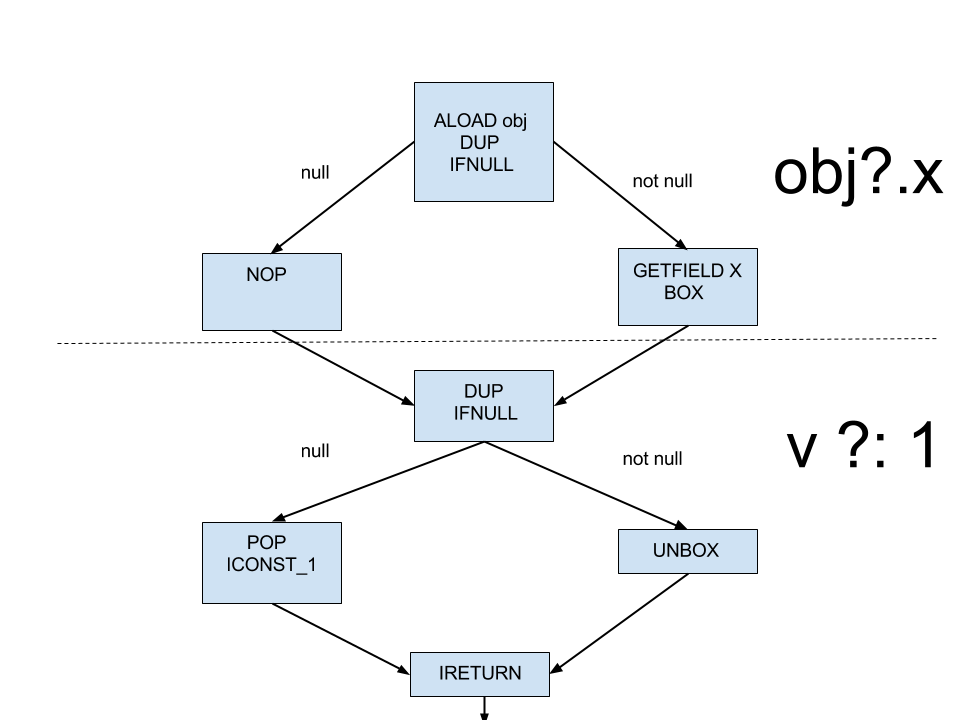
\includegraphics[scale=0.4]{../resources/safecall_elvis.png}
\end{center}
\caption{Блок-схема байт-кода для выражения ``return (obj?.x ?: 1)''}
\label{sc:elvis}
\end{figure}

Примерная блок-схема байт-кода бенчмарка изображена на рисунке \ref{sc:elvis}.
Часть, расположенная выше пунктирной линии описывает генерацию безопасного вызова:
\begin{itemize}
    \item На стек загружается переменная ``obj'', ее значение копируется с помощью инструкции
    ``DUP'', и копия проверяется на равенство ``null''.
    \item В случае если ``obj'' является нулевой ссылкой, то лежащее на вершине стека значение
    тоже нулевая ссылка.
    Иначе на стеке лежит объект ``obj'', у которого берется значение в поле ``x'' и упаковывается.
\end{itemize}

Таким образом обеспечивается контракт безопасного вызова, и на вершине стека находится либо нулевая
ссылка, либо упакованное значение поля.

Боксинг в данном случае необходим, так как ситуация, когда при одном потоке исполнения в ячейке
стека значение примитивного типа, а при другом --- ссылка, запрещена спецификацией виртуальной
машины\cite{JVMSpec}.

Вторая часть блок-схемы иллюстрирует байт-код для elvis-оператора:
\begin{itemize}
    \item Значение, лежащее на вершине стека, копируется и проверяется на равенство нулевой ссылке.
    \item В случае, если оно является нулевой ссылкой, то его копия снимается со стека и
    загружается значение по умолчанию --- целочисленная константа <<1>>.

    Иначе не стеке лежит объект класса ``java.lang.Integer'', из которого и получается значение
    с помощью вызова метода ``intValue'', на блок-схеме этот вызов отмечен для простоты, как
    ``UNBOX''.
\end{itemize}

Понятно, что байт-код этих операторов по отдельности наиболее очевидным образом выражает
их семантику, и выразить их еще проще в рамках спецификации JVM, пожалуй, не представляется
возможным.
Однако их сочетание ни в коей мере оптимальным не кажется.

\begin{figure}
\begin{center}
    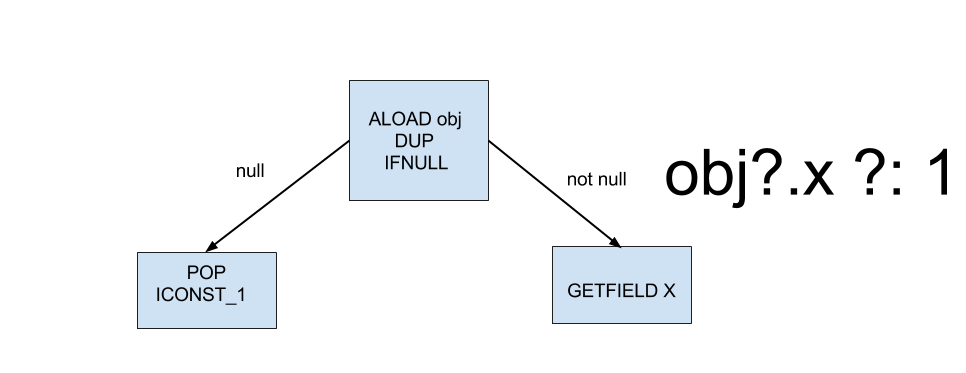
\includegraphics[scale=0.4]{../resources/safecall_elvis_optim.png}
\end{center}
\caption{Блок-схема байт-кода для выражения ``return (obj?.x ?: 1)'' (оптимальный вариант)}
\label{sc:elvisOpt}
\end{figure}

Наиболее кратким вариантом трансляции кажется изображенный на рисунке \ref{sc:elvisOpt}:
\begin{itemize}
    \item Переменная ``obj'' загружется на стек, создается ее копия, и сравнивается с нулевой
    ссылкой.
    \item Если значение является нулевой ссылкой, то его копия снимается со стека, и загружается
    значение по умолчанию.
    Иначе на вершине стека хранится объект, у которого берется значение поля ``x''.
\end{itemize}

При такой генерации отсутствуют операции боксинга, что, как выяснилось в рамках измерений,
хуже всего влияет на производительность вышеописанного байт-кода.

Оптимизации, направленные на решение найденной проблемы, описаны в разделе . % TODO: \ref

\subsubsection{Оператор when}
Оператор ``when'' в Kotlin является в некотором смысле расширением оператора ``switch'' в Java.
Если последний имеет ограниченный набор типов значений, для которых его можно использовать, то
``when'' определен для любых типов, и кроме сравнения на равенство его можно использовать для
проверки принадлежности чисел интервалу, или как некоторую разновидность паттерн-матчинга:

\begin{pyglist}[language=kotlin]
    when(x) {
        1, 2, 3, parseInt(s) -> print(1)
        in 4..1000 -> print(2)
        is String -> print(3)
        else -> print(4)
    }
\end{pyglist}
В случае неконстантных выражений-условий наиболее разумным способом генерации кажется простая
последовательная проверка истинности проверяемых выражений.
При трансляции байт-код для ``when'' аналогичен байт-коду цепочки ``if-else'' операторов,
производительность которых в Kotlin так или иначе не хуже аналогов из Java.

Важно отметить, что оператор ``switch'' можно применять только для набора выражений, которые можно
вычислить во время компиляции.
Причем при трансляции в байт-код используются специальные инструкции \textit{tableswitch} и
\textit{lookupswitch}\cite{JVMSpec}.
Их объединяет общая семантика:
\begin{itemize}
    \item Они параметризуются отображением из набора целых чисел в указатели на другие инструкции
    метода.
    \item При исполнении инструкции интерпретатор снимает с вершины стека число и совершает
    соответствующий переход.
\end{itemize}

Различия заключаются в том, что
\begin{itemize}
    \item \textit{tableswitch} параметризуется интервалом $[high..low]$.
    Для каждого целочисленного значения из этого интервала должна быть задана метка перехода,
    а кроме этого указатель на инструкцию по умолчанию.

    Таким образом размер этой инструкции линейно зависит от ширины интервала.
    \item \textit{lookupswitch} параметризуется отсортированным набором пар значений и меток
    перехода.

    Размер такой инструкции зависит линейно от числа значений.
\end{itemize}

Несмотря на то, что в спецификации не указана трудоемкость выполнения этих инструкций, из формата
их описания понятно, что ``tableswitch'' может быть исполнен за $O(1)$ прямым вычислением индекса
следующей инструкции, а ``lookupswitch'' может быть реализован на основе бинарного поиска и
работать за $O(log\ n)$.

На момент начала данного исследования эти инструкции не использовались в компиляторе Kotlin,
в связи с чем возникла необходимость оценить проигрыш в производительности для случая констант
времени компиляции по сравнению с Java.

Для этого был реализован следующий набор бенчмарков:
\begin{itemize}
    \item Функции с операторами ``switch''/``when'' с набором из последовательных значений
    для сопоставления из интервала $1..20$.
    Каждое условное ветвление представляет из себя оператор ``return'' с уникальным целым числом.
    Предполагается в Java такой ``switch'' транслируется в инструкцию ``tableswitch'',
    предзначначенную как раз для последовательных интервалов.

    \item Бенчмарки, аналогичные предыдущим, но с еще одним условным значением, значительно
    выходящим за пределы интервала $1..20$ --- $0$.
    Предполагается, что здесь должна быть использована инструкция ``lookupswitch'', подходящая
    для разреженных интервалов.

    \item Бенчмарки где операторы ``switch'' и ``when'' применяются для значений класса-перечисления
    (enum).
    Всего в классе объявлено 100 значений, в условном операторе используется 50 с четными номерами.

    \item Бенчмарки, где операторы ``switch'' и ``when'' применяются для строк.
    В качестве выражений для сопоставления использовались строки с вида <<ABCDEFGHIJKLMNO[i]>>,
    где $i$ --- порядковый номер в интервале $1..50$.

    В качестве аргументов использовались случайно выбранные строки из этого же множества.
\end{itemize}

Бенчмарки запускались в цикле на 1000 значений, выбранных случайным образом.

\begin{table}[h]
\begin{center}
\begin{tabular}{|c|c|c|c|} \hline
Разреженность & Java (мкс) & Kotlin (мкс) & Фактор \\ \hline
1..20 & 4.281 $\pm$ 0.018 & 7.8 $\pm$ 0.131 & 1.822\\ \hline
1..20, 100500 & 5.554 $\pm$ 0.077 & 7.524 $\pm$ 0.065 & 1.355\\ \hline
\end{tabular}
\caption{Сравнение производительности операторов switch/when для целочисленных констант}
\end{center}
\end{table}

\begin{table}[h]
\begin{center}
\begin{tabular}{|c|c|c|c|} \hline
Тип & Java (мкс) & Kotlin (мкс) & Фактор \\ \hline
Enum & 10.501 $\pm$ 0.167 & 13.885 $\pm$ 0.037 & 1.322\\ \hline
Строки & 21.667 $\pm$ 0.205 & 81.931 $\pm$ 1.671 & 3.781\\ \hline
\end{tabular}
\caption{Сравнение производительности операторов switch/when для классов перечислений и строк}
\end{center}
\end{table}

Из результатов измерений видно, что разница в производительности различных реализаций
составляет от $1.3$ до $3.7$ раз.

А так как использование константных выражений в подобного рода операторах является довольно
распространенной в программировании практикой, то при генерации следует рассмотреть такой
отдельно и при наличии возможность использовать оптимизирующие инструкции.

Подробности реализации оптимизации для данного случая можно рассмотреть в разделе . %% TODO: \ref

\subsubsection{Встраивание функций}
Изначально предполагается, что производительность встроенных функций должна быть аналогична
производительности кода, полученного при ручном встраивании.

Например код вызова:
\begin{pyglist}[language=kotlin]
    arrayOfInts.count { element -> element > 0 }
\end{pyglist}

где функция ``count'' определена как
\begin{pyglist}[language=kotlin]
    inline fun IntArray.count(predicate: (Int) -> Boolean): Int {
        var count = 0
        for (element in 0..size) {
            if (block(element)) {
                count++
            }
        }
        return count
    }
\end{pyglist}
не должен существенно уступать по производительности коду:
\begin{pyglist}[language=kotlin]
        var count = 0
        for (element in 0..size) {
            if (element > 0) {
                count++
            }
        }
\end{pyglist}

Однако, как было отмечено в разделе \ref{section:scala} добиться этого не слишком просто.

Для проверки влияния встраивания функций на производительность был реализован ряд бенчмарков,
каждый из которых проверяет эффективность различных функций стандартной библиотеки Kotlin
для работы с коллекциями:
\begin{itemize}
    \item ``count'' --- возвращает число элементов коллекции, удовлетворяющих заданному
    предикату-аргументу.
    \item ``filter'' --- возвращает ``ArrayList'' из значений коллекции, удовлетворяющих заданному
    предикату-аргументу.
    \item ``fold'' --- выполняет левоассоциативную свертку элементов коллекции, используя
    в качестве бинарной операции функцию-аргумент.
\end{itemize}

В качестве аргумента для функций использовался целочисленный массив, заполенный случайными числами.
Бенчмарки запускались для размеров массивов: 100, , 00.

В качестве эталонной версии использовался код, встроенный <<вручную>>, как в примере выше.

\begin{table}[h]
\begin{center}
\begin{tabular}{|c|c|c|c|} \hline
Размер & Эталон & Встроенная версия & Фактор \\ \hline
100 & 87.968 $\pm$ 0.78 нс & 348.255 $\pm$ 11.299 нс & 3.959\\ \hline
10000 & 18.401 $\pm$ 0.251 мкс & 78.05 $\pm$ 0.981 мкс & 4.242\\ \hline
1000000 & 3.715 $\pm$ 0.021 мс & 8.565 $\pm$ 0.098 мс & 2.306\\ \hline
\end{tabular}
\caption{Сравнение производительности вызова ``count \{ it \% 2 == 0 \}'' и аналогичного кода, встроенного вручную}
\label{bm:count}
\end{center}
\end{table}

\begin{table}[h]
\begin{center}
\begin{tabular}{|c|c|c|c|} \hline
Размер & Эталон & Встроенная версия & Фактор \\ \hline
100 & 598.23 $\pm$ 5.017 нс & 711.114 $\pm$ 8.057 нс & 1.189\\ \hline
10000 & 98.655 $\pm$ 1.764 мкс & 121.1 $\pm$ 1.74 мкс & 1.228\\ \hline
1000000 & 11.868 $\pm$ 0.529 мс & 13.68 $\pm$ 1.195 мс & 1.153\\ \hline
\end{tabular}
\caption{Сравнение производительности вызова ``filter \{ it \% 2 == 0 \}'' и аналогичного кода, встроенного вручную}
\label{bm:filter}
\end{center}
\end{table}

\begin{table}[h]
\begin{center}
\begin{tabular}{|c|c|c|c|} \hline
Размер & Эталон & Встроенная версия & Фактор \\ \hline
100 & 27.676 $\pm$ 0.159 нс & 477.024 $\pm$ 3.474 нс & 17.236\\ \hline
10000 & 2.784 $\pm$ 0.021 мкс & 47.563 $\pm$ 0.57 мкс & 17.084\\ \hline
1000000 & 301.023 $\pm$ 1.828 мкс & 4.69 $\pm$ 0.031 мс & 15.581\\ \hline
\end{tabular}
\caption{Сравнение производительности вызова ``fold(0) \{ sum, x -> sum + x \}'' и аналогичного кода, встроенного вручную}
\label{bm:fold}
\end{center}
\end{table}

Из результатов (см. таблицы \ref{bm:count}, \ref{bm:filter}, \ref{bm:fold}) видно, что код
встроенных версий от $1.$ до $16$ раз менее производительный, чем в принципе мог бы быть.

При профилировании с помощью плагина ``perfasm'' для JMH было установлено, что наибольший вред
для производительности приносит избыточный боксинг, оставшийся в качестве артефакта от встраивания
параметрически-полиморфного метода ``invoke'' анонимного класса (см. раздел \ref{section:lambda}).
Эта проблема так или иначе уже была поднята в рамках исследования\cite{ScalaDragos} и обсуждена
в рамках раздела \ref{section:scala}.

Наименее всего это влияет на бенчмарк ``filter'', так как значения все равно должны быть запакованы
перед сохранением в ''ArrayList``.

Сильнее всего разница заметна в случае бенчмакр ``fold'', где вычисляется сумма элементов массива.
Это связано с тем, что более чистый байт-код версии, написанной вручную, позволяет компилятору
HotSpot выполнить т.н. размотку цикла, суммирая в каждой итерации по $10$ элементов массива.

Оптимизации, связанные с улучшением производительности встраиваемых функций, описаны в разделе . %% TODO: \ref

\subsubsection{Замена на стеке}
Одной из разновидностей динамической трансляции, реализованной в Hotspot, является так называемая
<<Замена на стеке>> или ``On stack replacement''(OSR), описанная в \cite{HotspotServer}.

В отличие от простой версии JIT-компиляции, когда оптимизированная версия метода используется
только при следующем его вызове, OSR позволяет перейти к исполнению скомпилированного кода в рамках
уже начатого вызова.

Это может быть полезно, например, в случае, когда метод, содержащий цикл с трудоемкими вычислениями,
начал исполняться в режиме интерпретации, и при этом число итераций этого цикла достаточно велико.
В этом случае, если количество итераций преодолело порог-параметр ``OnStackReplaceThreshold'',
код метода компилируется, и в рамках следующей итерации исполняется оптимизированная версия.

Как следует из примера выше, для измерения времени работы необходим бенчмарк, содержащий долго
работающий цикл.
Такими бенчмарками могут послужить описанные в предыдущем разделе при больших размерах массива,
во время анализа работы которых было обнаружено странное поведения при компиляции метода на стеке.

А именно, функция ``foldBenchmark'' вида:
\begin{pyglist}[language=kotlin]
    fun foldBenchmark(): Int {
        return array.fold(0) { (x, y) -> x + y }
    }
\end{pyglist}

за разумное время компилировался <<на стеке>>, и хотя время его работы примерно в 20 раз
отличалось от эталонного, это можно было объснить избыточным боксингом.

Однако байт-код для семантически схожей функции ``foldBenchmarkOSR'' оказался в десятки раз менее
производительным, чем предыдущий (см. таблицы \ref{bm:foldOSR}, \ref{bm:foldOSR2}).
\begin{pyglist}[language=kotlin]
    fun foldBenchmarkOSR(bh: Blackhole) {
        bh.consume(array.fold(0) { (x, y) -> x + y })
    }
\end{pyglist}

Особенно интересным фактом в результатах измерений является то, что производительность второй
версии не уступает обычной версии ``fold'' при малых размерностях.
А кроме того, такое различие наблюдается только при запуске на версиях Hotspot 1.7, 1.8, когда
время на Hotspot 1.6 не отличается (см. таблицу \ref{bm:foldOSR3}).

\begin{table}[h]
\begin{center}
\begin{tabular}{|c|c|c|c|} \hline
Размер & Эталон & foldBenchmarkOSR & Фактор \\ \hline
100 & 27.832 $\pm$ 0.341 нс & 595.958 $\pm$ 4.061 нс & 21.413\\ \hline
10000 & 2.773 $\pm$ 0.006 мкс & 95.095 $\pm$ 0.832 мкс & 34.297\\ \hline
1000000 & 301.701 $\pm$ 4.575 мкс & 114.624 $\pm$ 2.055 мс & 379.925\\ \hline
\end{tabular}
\caption{Сравнение производительности вызова ``foldBenchmarkOSR'' и аналогичного кода, встроенного вручную (версия Hotspot 1.7)}
\label{bm:foldOSR}
\end{center}
\end{table}

\begin{table}[h]
\begin{center}
\begin{tabular}{|c|c|c|c|} \hline
Размер & fold & foldBenchmarkOSR & Фактор \\ \hline
100 & 594.34 $\pm$ 6.472 нс & 595.958 $\pm$ 4.061 нс & 1.003\\ \hline
10000 & 100.181 $\pm$ 0.584 мкс & 95.095 $\pm$ 0.832 мкс & 0.949\\ \hline
1000000 & 11.28 $\pm$ 0.063 мс & 114.624 $\pm$ 2.055 мс & 10.162\\ \hline
\end{tabular}
\caption{Сравнение производительности вызова ``foldBenchmarkOSR'' и аналогичного кода из бенчмарка ``fold'' (версия Hotspot 1.7)}
\label{bm:foldOSR2}
\end{center}
\end{table}

\begin{table}[h]
\begin{center}
\begin{tabular}{|c|c|c|c|} \hline
Размер & fold & foldBenchmarkOSR & Фактор \\ \hline
100 & 477.024 $\pm$ 3.474 нс & 478.739 $\pm$ 5.202 нс & 1.004\\ \hline
10000 & 47.563 $\pm$ 0.57 мкс & 47.482 $\pm$ 0.422 мкс & 0.998\\ \hline
1000000 & 4.69 $\pm$ 0.031 мс & 4.685 $\pm$ 0.051 мс & 0.999\\ \hline
\end{tabular}
\caption{Сравнение производительности вызова ``foldBenchmarkOSR'' и аналогичного кода из бенчмарка ``fold'' (версия Hotspot 1.6)}
\label{bm:foldOSR3}
\end{center}
\end{table}
Причем различия заметны только при больших размерностях задачи, что и дает повод искать корни
проблемы в трансляции <<на стеке>>, так как вероятно метод не успевает запуститься достаточное
число раз для полной компиляции.

После анализа журналов компиляции было определено, что компилятор Hotspot версий 7 и 8
не поддерживает для <<замены на стеке>> циклы, в начале которых стек виртуальной машины не пуст.

\begin{quote}
\begin{verbatim}
<failure reason='OSR starts with non-empty stack'/>
<failure reason='OSR starts with non-empty stack' phase='compile'/>
\end{verbatim}

\captionof{floatquote}{Фрагмент журналов компиляции}
\end{quote}

\begin{verbatim}

\end{verbatim}

Такая ситуация, когда цикл начинается с непустым стеком принципиально невозможна в Java, где
цикл не может быть частью выражения.

Однако проблема может возникнуть в языках, таких как Scala и Kotlin, где любые операторы являются
также и выражениями, то есть пример, описанный ниже --- корректная синтаксическая конструкция:
\begin{pyglist}[language=kotlin]
    fun foldBenchmarkOSR(bh: Blackhole) {
        foo().bar(for (i in 1..100) { print(i) })
    }
\end{pyglist}

Так как результат выражения ``foo()'' должен быть вычислен до выполнения аргумента вызова
``bar()'', то перед началом цикла на вершине стека находится результат ``foo()'', что и приводит
к невозможности проведения замены на стеке.

Несмотря на то, что использование цикла внутри выражения не имеет смысла, аналогичная ситуация
возникает и в разумных случаях, таких как в бенчмарке ``foldBenchmarkOSR'', где перед началом
цикла встроенной функции ``fold'' на стеке загружена переменная ``bh''.

Аналогичная проблема возникает и при встраивании функций в Scala\fu{https://issues.scala-lang.org/browse/SI-8057}.
Оптимизации, связанный с найденной проблемой описаны в разделе . %% TODO: \ref

\newpage
\section{Изменения в компиляторе}
В рамках данной главы будут описаны изменения в компиляторе, направленные на решение проблем,
найденных в разделе \ref{section:benchmarks}.

Исходные коды компилятора, в том числе изменения, описанные в данной работе, располагаются в
git-репозитории по адресу\cite{Kotlin}.

\subsection{Архитектура компилятора}
Большинство современных компиляторов, включая Kotlin, реализуют архитектурный шаблон, описанный
в \cite{Muchnick}.

Его суть состоит в разделении всего кода на следующие компоненты, каждая из которых должна зависеть
только от предыдущих:
\begin{enumerate}
    \item \textit{Лексический анализатор} --- принимает на вход содержимое программы в виде строки
    символов, и выдает поток семантически значимых фрагментов, т.н. <<токенов>>.

    \item \textit{Синтаксический анализатор} --- реализует один из алгоритмов синтаксического
    анализа и строит из потока <<токенов>> абстрактное синтаксическое дерево.

    \item \textit{Семантический анализатор}, получая абстрактное синтаксическое дерево, производит
    вывод типов выражений, если это необходимо, и проверяет корректность программы с точки зрения
    спецификации языка и его системы типов.

    \item \textit{Генератор кода} --- подсистема, генерирующая по размеченному синтаксическому
    дереву код для целевой архитектуры, в случае Kotlin --- class-файлы виртуальной машины Java.
\end{enumerate}

Для данной работы наибольший интерес, очевидно, представляет именно генератор кода.
Его часть, отвечающая за генерацию байт-кода методов представлена в виде класса, реализующего
шаблон проектирования <<Посетитель>>\cite{Gamma}, каждый ``visit''-метод которого отвечает за
генерацию отдельного вида узлов синтаксического дерева и чаще всего выполняет контракт,
гарантирующий, что результат аргумента-выражения окажется на вершине стека.

\subsection{Безопасный вызов и elvis-оператор}
\label{section:elvis:op}
%\begin{verbatim}
                %aload_1 // Загрузка `obj` на стек
                %dup
                %ifnull l1
                %getfield x
                %invokestatic  java/lang/Integer.valueOf() // Боксинг
                %goto          l3
                %l1: pop
                %aconst_null
                %// начало кода elvis-оператора
                %l2: dup
                %ifnull l3
                %invokevirtual java/lang/Number.intValue() // Распаковка
                %goto          l4
                %l3: pop
                %iconst_1
                %l4: ...
%\end{verbatim}

В разделе \ref{section:elvis:bm} были описаны произведенные измерения, демонстрирующие низкую
производительность байт-кода для сочетания безопасного вызова и elvis-оператора.

Ниже произведен более подробный анализ байт-кода бенчмарков и описаны решения для оптимизации.

\begin{figure}
\begin{center}
    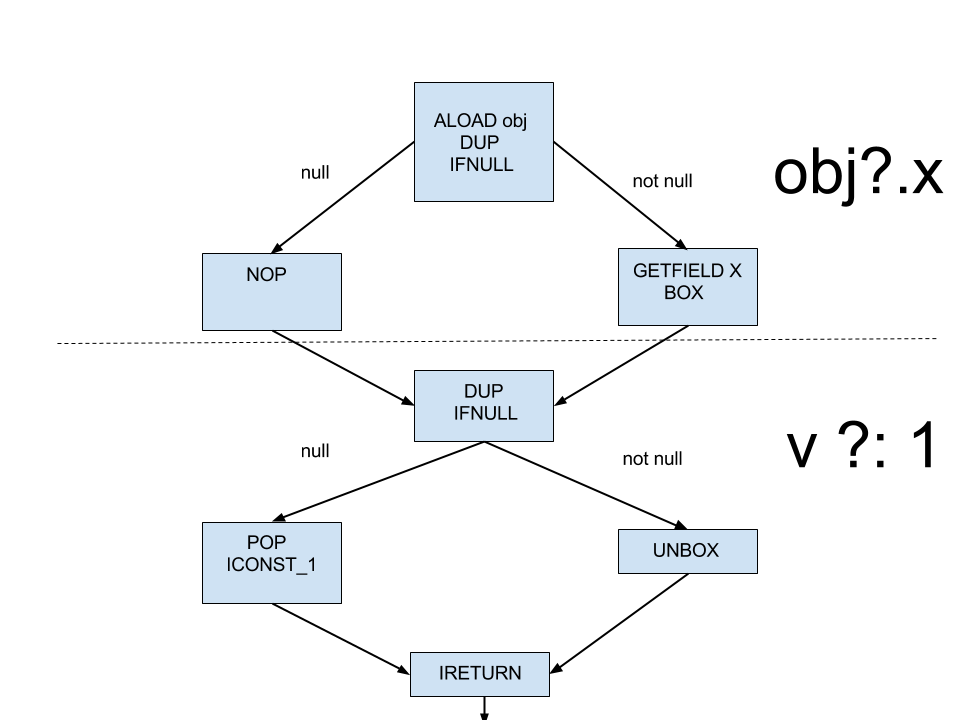
\includegraphics[scale=0.4]{../resources/safecall_elvis.png}
\end{center}
\caption{Блок-схема байт-кода для выражения ``return (obj?.x ?: 1)''}
\label{sc:elvis}
\end{figure}

Примерная блок-схема байт-кода бенчмарка изображена на рисунке \ref{sc:elvis}.
Часть, расположенная выше пунктирной линии описывает генерацию безопасного вызова:
\begin{itemize}
    \item На стек загружается переменная ``obj'', ее значение копируется с помощью инструкции
    ``DUP'', и копия проверяется на равенство ``null''.
    \item В случае если ``obj'' является нулевой ссылкой, то лежащее на вершине стека значение
    тоже нулевая ссылка.
    Иначе на стеке лежит объект ``obj'', у которого берется значение в поле ``x'' и упаковывается.
\end{itemize}

Таким образом обеспечивается контракт безопасного вызова, и на вершине стека находится либо нулевая
ссылка, либо упакованное значение поля.

Боксинг в данном случае необходим, так как ситуация, когда при одном потоке исполнения в ячейке
стека значение примитивного типа, а при другом --- ссылка, запрещена спецификацией виртуальной
машины\cite{JVMSpec}.

Вторая часть блок-схемы иллюстрирует байт-код для elvis-оператора:
\begin{itemize}
    \item Значение, лежащее на вершине стека, копируется и проверяется на равенство нулевой ссылке.
    \item В случае, если оно является нулевой ссылкой, то его копия снимается со стека и
    загружается значение по умолчанию --- целочисленная константа <<1>>.

    Иначе не стеке лежит объект класса ``java.lang.Integer'', из которого и получается значение
    с помощью вызова метода ``intValue'', на блок-схеме этот вызов отмечен для простоты, как
    ``UNBOX''.
\end{itemize}

Понятно, что байт-код этих операторов по отдельности наиболее очевидным образом выражает
их семантику, и выразить их еще проще в рамках спецификации JVM, пожалуй, не представляется
возможным.
Однако их сочетание ни в коей мере оптимальным не кажется.

\begin{figure}
\begin{center}
    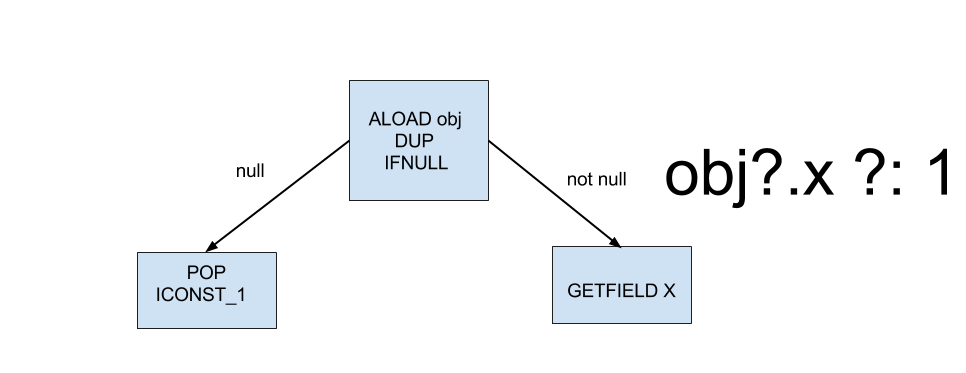
\includegraphics[scale=0.4]{../resources/safecall_elvis_optim.png}
\end{center}
\caption{Блок-схема байт-кода для выражения ``return (obj?.x ?: 1)'' (оптимальный вариант)}
\label{sc:elvisOpt}
\end{figure}

Наиболее кратким вариантом трансляции кажется изображенный на рисунке \ref{sc:elvisOpt}:
\begin{itemize}
    \item Переменная ``obj'' загружается на стек, создается ее копия, и сравнивается с нулевой
    ссылкой.
    \item Если значение является нулевой ссылкой, то его копия снимается со стека, и загружается
    значение по умолчанию.
    Иначе на вершине стека хранится объект, у которого берется значение поля ``x''.
\end{itemize}

При такой генерации отсутствуют операции боксинга, что, как выяснилось в рамках измерений,
хуже всего влияет на производительность вышеописанного байт-кода.

\paragraph{Решение}
В связи с условной оптимальностью байт-кода для операторов по отдельности, наиболее разумным
решением кажется специализация кодогенерации для выражений вида: $x_1?.x_2?...?.x_k\ ?: default$
в соответствие с идеей, проилюстрированной на рис. \ref{sc:elvisOpt}.

Упрощенно суть изменений можно выразить в виде следующего псевдокода:
\begin{lstlisting}[frame=single]
    function genElvis(v1: Expr, v2: Expr) {
        if (v1 is SafeCallChain) {
            // v1 ~ x1?.x2?...?.xk
            genSafeCallChain(v1, defaultLabel);
        } else {
            gen(v1);
        }

        DUP();
        IFNULL(defaultLabel);

        // ifNullLabel starts here
        gen(v2);
    }

    function genSafeCallChain(v: safeCallChain, ifNullLabel: Label) {
        for (element in v) {
            gen(v);
            DUP();
            IFNULL(ifNullLabel);
        }
    }
\end{lstlisting}

По сути логика генерации осталась прежней за исключением изменения генерации безопасных вызовов:
при проверке аргумента на равенство нулевой ссылке, сразу происходит переход к инструкции,
с которой начинается генерация значения по умолчанию.

Аналогичная оптимизация была произведена и для цепочки безопасных вызовов вне elvis-оператора,
в таком случае код можно генерировать по аналогии с выражением ``x1?.x2?..?.xk ?: null''.

В совокупности с изменениями, описанными в следующем разделе, это решение способствовало улучшению
производительности байт-кода, как микро-бенчмарков из раздела \ref{section:elvis:bm}, так и кода
АВЛ-дерева из раздела \ref{section:avl:bm}.
Результаты измерений в таблицах \ref{bm:elvis:o} и \ref{bm:stars:o}.

\begin{table}[h]
\begin{center}
\begin{tabular}{|c|c|c|c|c|} \hline
$p$ & Эталон (мкс) & До оптимизаций (мкс) & После оптимизаций (мкс) & Ускорение \\ \hline
0.1 & 4.693 $\pm$ 0.036 & 9.131 $\pm$ 0.126 & 4.619 $\pm$ 0.039 & 1.977\\ \hline
0.5 & 7.103 $\pm$ 0.078 & 7.138 $\pm$ 0.263 & 7.105 $\pm$ 0.039 & 1.005\\ \hline
0.9 & 4.561 $\pm$ 0.043 & 4.738 $\pm$ 0.047 & 4.523 $\pm$ 0.064 & 1.048\\ \hline
\end{tabular}
\caption{Результаты бенчмарка "Безопасный вызов и elvis" после оптимизаций \newline (p --- вероятность нулевой ссылки)}
\label{bm:elvis:o}
\end{center}
\end{table}

\begin{table}[h]
\begin{center}
\begin{tabular}{|c|c|c|c|c|} \hline
Размер & Java & Kotlin & После оптимизаций & Ускорение \\ \hline
100 & 19.412 $\pm$ 0.266 мкс & 30.687 $\pm$ 1.66 мкс & 21.837 $\pm$ 0.309 мкс & 1.405\\ \hline
1000 & 300.055 $\pm$ 2.397 мкс & 476.807 $\pm$ 4.243 мкс & 335.531 $\pm$ 11.768 мкс & 1.421\\ \hline
100000 & 78.686 $\pm$ 3.14 мс & 132.768 $\pm$ 3.938 мс & 79.394 $\pm$ 1.896 мс & 1.672\\ \hline
\end{tabular}
\caption{Результаты бенчмарка <<АВЛ-дерево>> после оптимизаций}
\label{bm:stars:o}
\end{center}
\end{table}

\subsection{Оператор when для константных выражений}
\label{section:when:opt}
Измерения, результаты которых изложены в разделе \ref{section:when:bm}, показали, что использование
байт-код инструкций ``tableswitch'' и ``lookupswitch'' для оператора ``when'' с константными
выражениями может значительно улучшить производительность соответствующего участка байт-кода.

Эти инструкции объединяет общая семантика:
\begin{itemize}
    \item Они параметризуются отображением из набора целых чисел в указатели на другие инструкции
    метода.
    \item При исполнении инструкции интерпретатор снимает с вершины стека число и совершает
    соответствующий переход.
\end{itemize}

Различия заключаются в том, что
\begin{itemize}
    \item \textit{tableswitch} параметризуется интервалом $[high..low]$.
    Для каждого целочисленного значения из этого интервала должна быть задана метка перехода,
    а кроме этого указатель на инструкцию по умолчанию.

    Таким образом, размер этой инструкции линейно зависит от ширины интервала.
    \item \textit{lookupswitch} параметризуется отсортированным набором пар значений и меток
    перехода.

    Размер такой инструкции зависит линейно от числа значений.
\end{itemize}

Несмотря на то, что в спецификации не указана трудоемкость выполнения этих инструкций, из формата
их описания понятно, что ``tableswitch'' может быть исполнен за $O(1)$ прямым вычислением индекса
следующей инструкции, а ``lookupswitch'' может быть реализован на основе бинарного поиска и
работать за $O(log\ n)$.

\paragraph{Выбор инструкции}
Сама по себе задача генерации специальных инструкций для случая, когда все выражения
для сопоставления в ``when'' --- константы, не представляется алгоритмически сложной, с учетом
наличия в компиляторе подсистемы для вычисления констант времени компиляции.

Однако существует некоторое количество тонкостей, о которых следует упомянуть в рамках данного
раздела.

Например при реализации неизбежно возникает проблема выбора между двумя инструкциями,
являющаяся по сути задачей многокритериального анализа:
\begin{itemize}
    \item ``tableswitch'' вероятно более производительна, но ее размер в байт-коде линейно
    пропорционален ширине интервала.
    \item ``lookupswitch'' более компактна, ее размер в байт-коде пропорционален числу меток.
\end{itemize}

В результате было принято решение воспользоваться эвристическим алгоритмом, который используется
для выбора инструкции в компиляторе Java из набора OpenJDK\fu{https://github.com/openjdk-mirror/jdk7u-langtools/blob/9f03d0c131f6343fee00f5dc5485c047e5cd2033/src/share/classes/com/sun/tools/javac/jvm/Gen.java\#L1159}:
\begin{itemize}
    \item Для каждого из вариантов вычисляется его условная стоимость как сумма стоимостей
    по памяти и производительности в виде числа сравнений --- $spaceCost + 3 * timeCost$

    \item Для ``tableswitch'' его стоимость по памяти полагается равной числу занимаемых машинных
    слов, т.е. $spaceCost = 4 + (high - low)$.

    Его трудоемкость оценивается значением $timeCost = 3$: два сравнения, необходимые для проверки,
    что данное число помещается в интервал $high..low$, и одно действие для безусловного прыжка.

    \item Для ``lookupswitch'': $spaceCost = 3 + 2 * n, timeCost = n$, где $n$ --- число меток.

    \item Вычисленные условные стоимости сравниваются и выбирается вариант с наименьшим
    результатом.
\end{itemize}

\paragraph{Оператор when для строк}
Для эффективного использования switch-инструкций, которые могут работать только с целочисленными
аргументами, при сравнении строк, используется хеш-функция, определенная в классе
``java.lang.String''.

Разумеется, из равенства значений хеш-функций нельзя делать выводы о равенстве строк,
поэтому в каждой метке switch-инструкции необходимо произвести соответствующие проверки.

Также следует обработать редкий случай, когда коллизии возникают между различными строками
из набора выражений для сопоставления.

Получаемый при генерации байт-код мог бы быть получен при компиляции следующего кода,
если бы в Java был реализован оператор ``goto''.
\begin{pyglist}[language=java]
String tmp0 = x;
switch(tmp0.hashCode()) {
    case 101584: if (tmp0.equals("foo")) { goto l1; }
    case 97299: if (tmp0.equals("bar")) { goto l2; }
}
l1: ...
l2: ...
\end{pyglist}

Любопытной деталью, является тот факт, что в компиляторе Java оператор ``switch'' для строк еще
до фазы генерации кода трансформируется в ``switch'' для целочисленных значений примерно такого же
вида, как изображенный выше код.
Однако ввиду отсутствия в языке конструкции ``goto'' его поведение эмулируется сохранением
во временную переменную номера совпавшей строки и дополнительным ``switch'' от этой переменной.

А так как изменения в компиляторе Kotlin производились внутри фазы кодогенерации, автору удалось
избавитсься от этой избыточности, и таким образом получить версию примерно на 10\% эффективней
версии Java (см. таблицу \ref{bm:switch:opt}).

\paragraph{Оператор when для enum-классов}
Для использования ``switch''-инструкций при генерации when для enum-классов использовался метод
``ordinal()`` определенный для каждой enum-константы, и возвращающий ее порядковый номер.

Однако компилятор Java выполняет дополнительную микрооптимизацию:
\begin{itemize}
    \item Для каждого класса, в котором вызывается ``switch'' от enum-класса, создается
    синтетический вложенный класс со статическими полями-массивами --- по одному на каждый такой
    ``switch''.
    \item Каждый массив имеет размер равный числу enum-констант в конкретном классе, и имеет смысл
    отображения порядковых номеров констант, используемых в метках, в последовательные номера
    от единицы.
    \item И вместо ``switch'' по непосредственному значению ``ordinal()`` генерируется ``switch''
    по элементу в соотвествующем массиве с индексом ``ordinal()''
\end{itemize}

Эта оптимизация, как следует из комментария к исходному коду, направлена на то, чтобы гарантировать
эффективное использование ``tableswitch'' при генерации оператора ``switch'' для enum-классов.

Реализация оптимизации ``when'' в Kotlin была сделана аналогично, в результате чего получаемый
байт-код можно проиллюстрировать следующим кодом на Java:
\begin{pyglist}[language=java]
    switch(CurrentClass$Mappings.$Mapping0[x.ordinal()]) {
        case 0: // ...
        case 1: // ...
        ...
    }
\end{pyglist}

\paragraph{Измерения после оптимизаций}
После внедрения описанных выше оптимизаций результаты бенчмарков, описанных
в разделе \ref{section:when:bm}, стали аналогичным результатам эталонных версий, написанных
на Java, кроме бенчмарка со строками, который стал производительней <<эталонного>> варианта на 10\%.

\begin{table}[h]
\begin{center}
\begin{tabular}{|c|c|c|c|c|} \hline
Разреженность & Java (мкс) & Kotlin (мкс) & После оптимизаций (мкс) & Ускорение \\ \hline
1..20 & 4.281 $\pm$ 0.018 & 7.8 $\pm$ 0.131 & 4.284 $\pm$ 0.029 & 1.821\\ \hline
1..20, 100500 & 5.554 $\pm$ 0.077 & 7.524 $\pm$ 0.065 & 5.55 $\pm$ 0.068 & 1.356\\ \hline
\end{tabular}
\caption{Сравнение производительности операторов switch/when для целочисленных констант после оптимизаций}
\end{center}
\end{table}

\begin{table}[h]
\begin{center}
\begin{tabular}{|c|c|c|c|c|} \hline
Тип & Java (мкс) & Kotlin (мкс) & После оптимизаций (мкс) & Ускорение \\ \hline
Enum & 10.501 $\pm$ 0.167 & 13.885 $\pm$ 0.037 & 10.476 $\pm$ 0.086 & 1.325\\ \hline
Строки & 21.667 $\pm$ 0.205 & 81.931 $\pm$ 1.671 & 19.295 $\pm$ 0.117 & 4.246\\ \hline
\end{tabular}
\caption{Сравнение производительности операторов switch/when для классов перечислений и строк после оптимизаций}
\label{bm:switch:opt}
\end{center}
\end{table}

\subsection{Постобработка байт-кода}
В рамках анализа результатов запусков бенчмарков был выявлен класс проблем, которые было бы сложно
решать в рамках фазы кодогенерации, а именно избыточный боксинг (см. \ref{section:inline:bm}) и
нарушения условия для выполнения OSR (\ref{section:osr:bm}).

Основная сложность заключается в том, что корень этих проблем лежит во встраивании функций ---
механизме, который работает с уже сгенерированным байт-кодом (встраиваемой функции), причем
семантика встраиваемого кода хотя бы в виде исходников для подсистемы встраивания недоступна,
что затрудняет оптимизации на этой фазе, и так или иначе приводит к необходимости постобработки
байт-кода.

Надо отметить, что избавление от артефактов встраивания в отдельной фазе компиляции ни в коей мере
не является чем-то новым и обсуждается, как в известной литературе\cite{Muchnick}, так и в работе
про оптимизации в Scala\cite{ScalaDragos}.

\subsubsection{Абстрактная интерпретация}
Абстрактная интерпретация или ее частный случай --- анализ потока данных --- являются наиболее
часто используемыми подходами при постобработке сгенерированного кода и при реализации
различных вариантов статического анализа.

С их помощью можно проверять или выводить те или иные утверждения о программном коде в самых разных
его аспектах.

Здесь описывается общий каркас для алгоритмов анализа потока данный, изложенный частично в \cite{Muchnick}
и \cite{Nielson}.

Основная суть этого подхода заключается в представлении процедуры в виде графа, где вершины ---
базовые блоки --- отдельные инструкции промежуточного языка или непрерывно исполняемые участки
программы, а ребра --- возможные переходы между ними.
Ориентация ребер зависит от вида анализа, который бывает \textit{прямым} или \textit{обратным}.

Еще одним важным элементом анализа является решетка
$$\mathbb{T} = (\mathbb{T}, \sqsubseteq, \bigsqcup, \bigsqcap, \top, \bot)$$
определяющая состояние программы в каждом базовом блоке.

Операция $\bigsqcup$ определяет состояние, возникающее в результате слияния других состояний.

Нередко в качестве состояния программы подразумевают состояние ее ячеек памяти, тогда в качестве
решетки удобно взять вектор $\mathbb{T} :: = StackState = (\mathbb{X}^v)$, где $v$ --- число ячеек
памяти, а $\mathbb{X}$ --- некоторая другая решетка.

Также для каждого базового блока задают монотонную трансфер-функцию
$transfer_b :: \mathbb{T} \to \mathbb{T}$, отражающую семантическое влияние блока на состояние программы
при его исполнении.
Монотонность трансфер-функции необходима для сходимости алгоритма и чаще всего очевидна.

Далее строится система уравнений --- по два на каждый блок $b$:
$$in_b: \mathbb{T} ::= \bigsqcup \{out_x\ |\ x \in pred_b\}$$
$$out_b: \mathbb{T} ::= transfer_b(in_b)$$

Также эту систему удобно представить в виде векторной функции: $F :: \mathbb{T}^{2n} \to \mathbb{T}^{2n}$

Решение этой системы так или иначе отвечает на вопрос, какие состояния в принципе могут быть
актуальны в различных точках программы.
Однако чаще всего интересует ответ на вопрос о минимальном решении, т.к. обычно решетка строится
так, что меньшие элементы являются условно более точными.
Его определяют как:
$$lfp(F) = \bigsqcap Fix(F) =  \bigsqcap\{ x | F(x)= x\}$$

Из определения очевидна минимальность полученного вектора из тех, которые в принципе могут быть
решениями, а из теоремы Тарского следует что результат будет неподвижной точкой, а кроме
того в виде следствия дается алгоритм для его вычисления: $lfp(F) = F^n(\bot)$, где $n \to \infty$.

Причем для конечных решеток с учетом монотонности $F$ очевидна сходимость алгоритма за конечное
число шагов.

\subsubsection{Архитектура подсистемы}
В рамках реализации подсистемы постобработки для работы с байт-кодом, и для реализации алгоритмов
анализа потока данных использовались существенные части библиотеки ASM\fu{http://asm.ow2.org/}.

Она предоставляет набор инструментов для работы с class-файлами, байт-кодом методов и каркас,
реализующий общую часть алгоритма анализа потока данных.

ASM предлагает весьма удобную абстракцию для представления байт-кода метода --- класс
``MethodNode'', в котором с множеством инструкций можно обращаться, как с обычным изменяемым
списком, а отдельные инструкции представлены в виде классов с удобным интерфейсом доступа
к их аргументам. Например инструкции переходов хранятся как объекты класса ``JumpInsnNode'',
в котором в качестве поля содержится ссылка на инструкцию, куда может быть произведен переход.

\paragraph{Каркас алгоритма анализа потока данных}
Также, как уже было сказано выше, библиотека предоставляет базовую реализацию алгоритмов, которые
в частности можно использовать и для анализа потока данных и потока управления в виде каркаса.

Для его использования разработчику следует:
\begin{itemize}
    \item Создать класс, реализующий интерфейс ``Value''. Объекты этого класса как раз и будут
    элементами решетки $\mathbb{X}$, описанной в предыдущем разделе.

    \item Реализовать интерфейс ``Interpreterer'', методы которого как раз описывают трансфер-функцию
    для каждого типа инструкций.
    Кроме того, здесь же необходимо определить операцию $\bigsqcup$ для двух элементов
    решетки, реализовав метод ``merge''.

    \item После чего создается объект класса ``Analyzer'', реализующий логику поиска наименьшего
    решенияи параметризуется конкретными реализациями ``Value'' и ``Interpreter''.

    Метод ``analyze'' принимает объект ``MethodNode'' и возвращает массив из объектов ``Frame'',
    каждый из которых содержит информацию о состоянии стек-фрейма для каждой из инструкций метода.

    В классе ``Frame'' реализованы методы ``getLocal''/``getStack'', возвращающие элемент решетки,
    находящийся в полученном решении в конкретной локальной переменной или на определенном сдвиге
    от вершины стека.
\end{itemize}

Следует однако уточнить, что предложенный в библиотеке каркас обладает рядом недостатков:
\begin{itemize}
    \item Для его корректной работы требуется точное вычисление максимального размера стека
    в методе, а также числа используемых переменных.

    Для автора данной работы остаются загадкой причины, по которым вычисление этих величин
    не производится в рамках анализа самим каркасом.
    Причем единственное место в библиотеке, где эта логика реализована --- подсистема генерации
    бинарного представления class-файла.

    Таким образом у разработчиков остается два варианта: искусственно генерировать бинарное
    представление метода, откуда можно получить эти величины, или в своем коде дублировать логику
    их вычисления, что в общем случае не тривиально.
    Автором был выбран второй подход, так как он значительно менее ресурсоемок.

    \item Еще одной существенной проблемой каркаса является его недостаточная гибкость:
    \begin{itemize}
        \item Аналогам трансфер-функций доступен не весь стек-фрейм, а только та его часть,
        которая относится к конкретной инструкции, чего не всегда бывает достаточно.

        \item Для некоторых видов инструкций, таких как ``POP'' --- просто снимающих значение
        с вершины стека --- не предусмотрены трансфер-функции, и их обработку можно произвести
        только в формате дополнительного анализа, запустив его после основного.

        \item Элементы стека в классе ``Frame'' неизменяемыми, единственное, что возможно ---
        удалять элемент с вершины стека, и добавлять новый.
    \end{itemize}

    \item Каркас предоставляет возможность только для <<прямого>> анализа, таким образом его
    невозможно использовать например для определения интервалов времени жизни переменных.
\end{itemize}

Однако для решения задач анализа, поднятных в рамках данной работы, функциональности библиотеки
в целом было достаточно, поэтому описанные далее алгоритмы так или иначе были реализованы
с помощью этого каркаса.

\paragraph{Внедрение в компилятор}
Одним из тривиальных, но тем не менее важных пунктов работы, стала задача внедрения в компилятор
подсистемы постобработки байт-кода.

Сама разработанная подсистема состоит из двух частей:
\begin{itemize}
    \item Множество алгоритмов, так или иначе реализующих непосредственно логику изменения
    байт-кода.

    Каждый из них должен быть представлен в виде класса, реализующего абстрактный класс
    ``MethodTransformer'', содержащий единственный абстрактный метод ``transform'', принимающий
    ``MethodNode'' в качестве аргумента, в котором и должна быть описана содержательная часть
    алгоритма.

    Таким образом эта часть состоит из списка алгоритмов ``MethodTransformer'', которые в принципе
    должны быть независимы друг от друга, однако на деле важным оказывается порядок, в котором
    эти алгоритмы применяются к каждому из методов.

    \item Часть, взаимодействующая с подсистемой кодогенерации.
    Здесь можно вкратце сказать от том, что последняя оперирует с байт-кодом с помощью абстракции
    все той же библиотеки ASM --- MethodVisitor, и для добавления следующий инструкции в байт-код
    вызывается тот или иной метод этой абстракции.

    Поэтому для того, чтобы перед непосредственно записать в class-файл байт-код метода,
    выполнялась его пост-обработка необходимо было с помощью шаблона проектирования
    <<декоратор>>\cite{Gamma} реализовать свой вариант ``MethodVisitor'', аккумулирующий байт-код
    в ``MethodNode'', и при вызове ``endVisit'', запускающий процесс трансформации, результат
    которого передается в декорируемый ``MethodVisitor''.

    Этой реализацией необходимо заместить существующую, которая создается при создании нового метода
    в классе ``ClassBuilder''.

    Более подробно можно рассмотреть полученное архитектурное решение в диаграмме классов [?]. % TODO:
\end{itemize}

\subsubsection{Удаление избыточного боксинга}
В рамках раздела \ref{section:inline:bm} было выявлено одно из проблемных мест при встраивании
функций, а именно наличие избыточного боксинга.

Для начала необходимо определить и зафиксировать понятия <<боксинга>> и его <<избыточности>>.

\textit{Боксингом} назовем получение объекта одного из классов-оболочек для хранения примитивных
типов (см. раздел \ref{section:lambda}) по имеющемуса примитивному значению.
Чаще всего это происходит в результате вызова статического метода ``valueOf'' у этих классов.

\textit{Избыточной} назовем операцию боксинга, результат которой --- объект класса-оболочки ---
используется только для условно <<чистых>> операций:
\begin{itemize}
    \item Сохранение или загрузка значения в локальную переменную.
    \item Cтандартные операции на стеке: POP/DUP.
    \item Инструкции уточняющие информацию о значении на вершине стека: IFNULL, IFNONNULL,
    CHECKCAST, INSTANCEOF.
    \item Вызовы методов, возвращающие хранимое значение примитивного типа, например
    ``Integer.intValue()''.
    \item Вызовы методов для конвертации запакованного значения к типам других примитивов,
    например метод ``Integer.longValue()''.
\end{itemize}

Суть этих требований проста:
\begin{itemize}
    \item Если значение, полученное в результате боксинга используется в рамках других инструкций,
    например вызов метода ``hashCode'', то очевидно, что операция упаковки неизбежно должна иметь
    место до этого вызова.

    \item С другой стороны все перечисленные операции действительно либо могут быть удалены, как
    в случае с инструкцией IFNULL --- так как известно, что запакованное значение не может быть
    равно нулевой ссылке, либо могут быть заменены на аналогичные операции с примитивами:
    ASTORE $\to$ ISTORE, ``Integer.longValue()'' $\to$ I2L.
\end{itemize}

Также необходимо, чтобы при любом пути исполнения метода не возникало ситуации, когда в том же
слоте стек-фрейма, где хранится запакованное значение, которое потенциально <<избыточно>>
не могло теоретически оказаться:
\begin{itemize}
    \item Другого объекта ссылочного типа. Как минимум причиной для такого требования может служить
    спецификация виртуальной машины, запрещающая разделение слота значениями различной природы.
    Кроме того, в результате смешивания значений должен наблюдаться специфический результат,
    например в коде ниже в зависимости от условия должна сохраняться возможность исключения
    ``NullPointerException'':
    \begin{pyglist}[language=kotlin]
        val x = if (cond) Integer.valueOf(1) else null
        x.intValue() // Possible NullPointerException
    \end{pyglist}

    \item Объекта полученного в результате боксинга другого типа, например Integer и Long.

    Это связано с тем, что при потенциальной возможности такого слияния, заменить значения на
    примитивы не удастся опять же в связи с тем, что это запрещено спецификацией.

    \item Значения, полученного в результате боксинга, которое не может быть удалено.
\end{itemize}

Таким образом боксинг можно назвать \textit{избыточным} тогда и только тогда, когда полученное
значение используется только как операнд для <<чистых>> инструкций и любое значение, с которым
первое значение может разделять место в стек-фрейме является запакованным значением такого же
типа, боксинг которого можно назвать \textit{избыточным}.

Отметим, что определение получилось рекурсивным.

\paragraph{Специализированные итераторы}
В Kotlin определены специализированные версии итераторов для каждого из примитивных типов:
``IntIterator'', ``FloatIterator'' и т.д.

Каждый из них является абстрактным классом, требующим реализации метода вида ``nextT'', например
``nextInt'':
\begin{pyglist}[language=kotlin]
    public abstract class IntIterator : Iterator<Int> {
        override final fun next() = Integer.valueOf(nextInt())
        public abstract fun nextInt(): Int
    }
\end{pyglist}

Важно отметить, что такие итераторы реализуют более общий параметрически-полиморфный интерфейс
``Iterator<T>'', где возникает необходимость в боксинге значения.

Наиболее часто встречающимися примерами реализации таких итераторов являются итераторы
по числовому отрезку. Синтаксически выраженные как $(low..high)$, при трансляции в JVM они
становятся объектами классов ``<T>Range'', где T --- один из числовых примитивов, которые можно
использовать как обычные неизменяемые коллекции, например:
\begin{pyglist}[language=kotlin]
    (1..100).count { it % 2 == 0 }
\end{pyglist}

Причем в качестве итераторов возвращаются как раз объекты специализированных классов, однако
большая часть библиотечных функций, включая ``count'' из примера, работают с ними, как с обычными
итераторами, вызывая метод ``next'', который также можно считать операцией боксинга наравне
с вызовами ``valueOf''.

Таким образом необходимо также анализировать является ли объекты, ссылки на которые хранятся
в стек-фрейме, специализированными итераторами или объектами классов "<T>Range".

\paragraph{Определение решетки}
Таким образом множество элементов решетки можно задать так:
$$\mathbb{X} = \{\bot = Nothing \sqsubseteq  Primitive, Boxed, Range, PrimitiveIterator \sqsubseteq \top = Object \}$$
Здесь
\begin{itemize}
    \item $\top = Object$ --- произвольное значение ссылочного типа.
    \item $\bot = Nothing$ --- неинициализированное значение, в частности необходимое для полноты
    решетки.
    \item $Primitive$ --- значение примитивного типа.
    \item $Boxed$ --- ссылочное значение, полученное в результате боксинга.
    \item $Range$ --- ссылочное значение, являющееся объектом вида $(low..high)$.
    \item $PrimitiveIterator$ --- ссылка, указывающая на специлизированный итератор.
\end{itemize}

Операция $\bigsqcup$ для двух элементов задается так:
$$x \bigsqcup y =
\begin{cases}
y & \text{if } x == \bot \\
x & \text{if } y == \bot \\
x & \text{if } x == y \\
Object & \textit{Иначе}
\end{cases}
$$

Под равенством элементов подразумевается, как эквивалентность элементов решетки, так и равенство
содержимых типов (для Boxed, Range, PrimitiveIterator).

Трансфер-функции для большей части случаев тривиальны, так как порождены семантикой инструкций.
Исключение составляют вызовы методов, продуцирующие новые значения специфичных типов:
\begin{itemize}
    \item \textit{transfer(INVOKESTATIC, WRAPPE\_CLASS, "valueOf(T)") = Boxed}
    \item \textit{transfer(INVOKESPECIAL, RANGE\_CLASS, "<init>") = Range}
    \item \textit{transfer(INVOKEINTERFACE, "iterator()") = PrimitiveIterator}, если аргумент вызова есть $Range$.
    \item \textit{transfer(INVOKEINTERFACE, "next()") = Boxed}, если аргумент вызова есть $PrimitiveIterator$.
\end{itemize}

Следует уточнить, что полученные трансфер-функции не являются функционально-чистыми, так как
в момент анализа аккумулируют список Boxed-значений, изменяют информацию о <<чистоте>> их
использования в случае <<неудачного>> слияния и так далее.

Таким образом в результате реализованный автором алгоритм анализа возвращает список Boxed-значений,
которые согласно определению выше являются избыточными, а также список инструкций, для
которых каждое из значений является операндом.

\paragraph{Адаптация инструкций}
После выяснения множества чистых Boxed-значений, необходимо адаптировать оперирующие
с ними инструкции для работы с аналогичными примитивами.

Например удалить операции ``CHECKCAST'', производящие принадлежность объекта классу, если результат
в любом случае положителен (например ``CHECKCAST Number'' применяемый к Integer), заменить
инструкции доступа к переменным ссылочного типа на соответствующие инструкции, работающие
с примитивами и т.д.

Также необходимо изменять информацию об изменении типа в таблице локальных переменных.
Это может быть несколько нетривиально в случае, когда тип меняется со ссылочного на примитив,
занимающий два слота памяти: ``long'' или ``double''.
В этом случае необходимо сдвигать индексы переменных, имеющих большие номера, причем изменять надо
как в таблицу, так и инструкции байт-кода.

\paragraph{Недостатки решения}
Предложенное решение обладает рядом незначительных недостатков.

Например, если запакованное значение в большинстве случаев используется только для получения
хранимого значения, и только в одном месте является операндом <<грязной>> инструкции, данный
алгоритм ничего не изменит.

Автор статьи про оптимизации компилятора Scala\cite{ScalaDragos} предлагает альтернативное
решение --- перед боксингом сохранять примитив во временную переменную, и использовать ее
значение каждый раз вместо процедуры <<распаковки>>.

Причем сама операция боксинга или эта временная переменная будет удалена последующим анализом
времени жизни переменных в случае их неиспользуемости.

Однако в статье не был подробно разобран момент слияния двух различных Boxed-значений:
кажется единственным вариантом в момент слияния создавать еще одну переменную, по аналогии с тем,
как это происходит с $\varphi$-функциями в $SSA$\cite{Muchnick}, что существенно усложняет
трудоемкость анализа, а кроме того добавляет потенциально лишние инструкции в байт-код.

Для оценки того, насколько часто в обычном коде встречаются такие сложные случае был реализован
оптимистичный анализ, детектирующий любые случаи боксинга, результат которых хотя бы раз
используется в методе для распаковки значения, т.е. потенциально избыточные.

Результат был запущен на нескольких проектах, написанных на Kotlin: реализации задач Project Euler,
Kannotator, Kara.
Всего было найдено около 600 искомых операций боксинга, из которых только 7 не могли быть удалены
описанным выше алгоритмом.
Таким образом предложенное решение позволяет избежать боксинга в большинстве найденных случаев.

\paragraph{Результаты}
После внедрения описанного решения в компилятор были проведены повторные измерения
производительности на бенчмарках со встраиваемыми функциями. Результаты приведены в таблицах
\ref{bm:count:opt}, \ref{bm:filter:opt} и \ref{bm:fold:opt}.

\begin{table}[h]
\begin{center}
\begin{tabular}{|c|c|c|c|c|} \hline
Размер & Эталон & До & После & Ускорение (раз) \\ \hline
100 & 87.968 нс & 348.255 нс & 88.63 нс & 3.929\\ \hline
10000 & 18.401 мкс & 78.05 мкс & 18.655 мкс & 4.184\\ \hline
1000000 & 3.715 мс & 8.565 мс & 3.711 мс & 2.308\\ \hline
\end{tabular}
\caption{Сравнение производительности вызова ``count \{ it \% 2 == 0 \}'' до и после оптимизаций}
\label{bm:count:opt}
\end{center}
\end{table}

\begin{table}[h]
\begin{center}
\begin{tabular}{|c|c|c|c|c|} \hline
Размер & Эталон & До & После & Ускорение (раз) \\ \hline
100 & 598.23 нс & 711.114 нс & 482.667 нс & 1.473\\ \hline
10000 & 98.655 мкс & 121.1 мкс & 97.938 мкс & 1.236\\ \hline
1000000 & 11.868 мс & 13.68 мс & 11.292 мс & 1.212\\ \hline
\end{tabular}
\caption{Сравнение производительности вызова ``filter \{ it \% 2 == 0 \}'' до и после оптимизаций}
\label{bm:filter:opt}
\end{center}
\end{table}

\begin{table}[h]
\begin{center}
\begin{tabular}{|c|c|c|c|c|} \hline
Размер & Эталон & До & После & Ускорение (раз) \\ \hline
100 & 27.832 нс & 594.34 нс & 27.928 нс & 21.281\\ \hline
10000 & 2.773 мкс & 100.181 мкс & 2.776 мкс & 36.092\\ \hline
1000000 & 301.701 мкс & 11.28 мс & 304.423 мкс & 37.054\\ \hline
\end{tabular}
\caption{Сравнение производительности вызова ``fold(0) \{ sum, x -> sum + x \}'' до и после оптимизаций}
\label{bm:fold:opt}
\end{center}
\end{table}

\subsubsection{Избыточные проверки на равенство null}
Еще один этап постобработки --- удаление избыточных проверок на равенство null.

Несмотря на то, что наличие таковых избыточных проверок в пользовательском коде нетипично, они
могут появляться при встраивании --- когда встраиваемая функция написана с расчетом на то, что
определенное значение может быть нулевой ссылкой, однако после встраивания можно доказать, что
это невозможно.

Также это может быть необходимо после генерации оператора приведения `as`, семантика которого
обязывает генерировать проверку на равенство null.

Рассматриваемый вид оптимизаций направлен не столько на увеличение производительности байт-кода,
так как сами по себе эти проверки не слишком трудоемки, хотя и могут отрицательно влиять на
предсказатель переходов ЦПУ, сколько для уменьшения размера получаемого байт-кода: удаление
таких проверок может делать недостижимыми большие участки кода.

\paragraph{Анализ}
Анализ предмет вывода возможности равенства нулевой ссылке различных значений
не является чем-то существенно новым в мире статического анализа JVM-байт-кода.
В данной работе реализована простая версия таких алгоритмов, также как и предыдущее решение,
основанная на фреймворке для анализа потока данных из библиотеки ASM.

Здесь используется похожая решетка значений, как и в случае анализа из предыдущего раздела:
$$\mathbb{X} = \{\bot = Nothing \sqsubseteq  Primitive, NotNull \sqsubseteq \top = Object \}$$

Здесь \textit{NotNull} --- значение про которое доказано, что оно содержит ссылку, не являющуюся
нулевой ссылкой.

Операция $\bigsqcup$ задается аналогично, с тривиальным уточнением:
$$x \bigsqcup y = NotNull \Leftrightarrow x = NotNull \land y = NotNull$$

Трансфер-функции снова тривиальны за исключением тех, которые порождают NotNull-значения:
\begin{itemize}
    \item ANEW, ANEWARRAY --- создающие новый объект или массив.
    \item LDC --- загружающая константу из пула констант.
    \item Инструкции, так или иначе, порождающие боксинг, гарантируют, что полученный объект
    не равен null.
\end{itemize}

Последний пункт порождает необходимость абстракции кода, вычисляющего множество Boxed-значений,
для его переиспользования в обоих случаях.

В свою очередь удаление всех таких избыточных проверок упрощает трансформацию кода для
удаление избыточного боксинга.

\paragraph{Трансформация байт-кода}
После получения результатов анализа для каждой инструкции IFNULL/IFNOTNULL в случае, если можно
доказать, что значение на вершине стека не равно null, то:
\begin{itemize}
    \item Значение снимается с вершины стека, добавление инструкции POP перед текущей.

    Это необходимо, чтобы размер стека после исполнения остался таким же, как и в случае
    с исходной инструкцией.

    \item Инструкция IFNULL просто удаляется, так как такой переход в любом случае не будет
    выполнен, а инструкция IFNOTNULL заменяется на безусловный переход --- GOTO к той же метке,
    что и в исходной инструкции.

    \item Дополнительная микрооптимизация состоит в том, что если инструкция перед POP не имеет
    посторонних эффектов при своем исполнении, например загрузка локальной переменной --- ASTORE,
    или копирование значения на вершине стека --- DUP, то можно, не добавляя искусственной инструкции
    POP, просто удалить предыдущую.
\end{itemize}

\subsubsection{Удаление недостижимого кода}
Один из результатов оптимизации, описанной в предыдущем разделе, состоит в порождении веток
недостижимого или <<мертвого>> кода.

В принципе мертвый код может порождаться и в других случаях, например с точки зрения системы типов
если тело функции состоит из вызова другой функции, имеющей тип ``Nothing'', то можно опустить
return-оператор, так как считается, что любое выражение, имеющее такой тип не может завершиться.

Однако с точки зрения виртуальной машины такой метод выглядит так, как будто в нем есть ветка
исполнения, в которое не вызывается инструкция RETURN, в связи с чем система кодогенерации
добавляет искусственную инструкцию RETURN в конец каждого метода, причем в большинстве
случае такие инструкции недостижимы.

Формальное определение недостижимости инструкции просто выводится из представления кода в виде
графа --- базовый блок, или инструкция называется недостижимой, если не существует пути
ведущего в этот блок из точки входа в процедуру.

Самый простым с точки зрения реализации способ разметить достижимость кода в рамках библиотеки ASM
является запуск стандартного анализатора, поставляемого вместе с библиотекой.

Гарантируется, что когда в полученном массиве фреймов элемент равен нулевой ссылке, то
соответствующая ему инструкция недостижима.

Найденные таким образом недостижимые инструкции просто удаляются из списка ``MethodNode''.


\clearpage
\section*{Заключение}
\addcontentsline{toc}{section}{\hspace{7mm}Заключение}

В рамках данной работы достигнуты следующие результаты:

\begin{enumerate}
    \item Автором было произведено исследование подходов, применяемых для оптимизации
    производительности байт-кода в других компиляторах под платформу Java.

    \item Реализован набор бенчмарков, измеряющих эффективность байт-кода генерируемого
    компилятором Kotlin.

    \item Проведен анализ измерений, полученных в результате запусков бенчмарков, выявлены
    проблемные места.

    \item Также описаны изменения, исправляемые найденные недостатки и успешно внедренные в компилятор:
    \begin{itemize}
        \item Специализирована генерация байт-кода оператора when для целочисленных констант, строк и enum-классов \\
        \textit{(ускорение от 1.3 до 4.3 раз)}

        \item Оптимизирован процесс генерации сочетания Elvis + Safe-call \\
        \textit{(ускорение от 1.4 до 1.7 раз)}

        \item В компилятор добавлена подсистема постобработки байт-кода.
        \item Реализовано решение для удаления избыточно боксинга \\
        \textit{(ускорение от 1.2 до 37 раз)}
        \item Решена проблема с нарушением условия для <<замены на стеке>> \\
        \textit{(ускорение до 379.3 раз)}
        \item Реализован алгоритм для удаления избыточных проверок на равенство ссылок null
        \item Добавлено решение для удаления недостижимого кода
    \end{itemize}
\end{enumerate}

Набор бенчмарков, реализованный в данной работе можно посмотреть в git-репозитории, расположенном
по адресу \url{https://github.com/bintree/kotlin-jmh-benchmarks}.

Адрес репозитория компилятора Kotlin: \url{https://github.com/JetBrains/kotlin}.


\newpage
\nocite{*}
\bibliographystyle{bplain}
\bibliography{biblio}

\end{document}

